% This is the Reed College LaTeX thesis template. Most of the work
% for the document class was done by Sam Noble (SN), as well as this
% template. Later comments etc. by Ben Salzberg (BTS). Additional
% restructuring and APA support by Jess Youngberg (JY).
% Your comments and suggestions are more than welcome; please email
% them to cus@reed.edu
%
% See https://www.reed.edu/cis/help/LaTeX/index.html for help. There are a
% great bunch of help pages there, with notes on
% getting started, bibtex, etc. Go there and read it if you're not
% already familiar with LaTeX.
%
% Any line that starts with a percent symbol is a comment.
% They won't show up in the document, and are useful for notes
% to yourself and explaining commands.
% Commenting also removes a line from the document;
% very handy for troubleshooting problems. -BTS


%%%%%%%%%%%%%%
%% Preamble %%
%%%%%%%%%%%%%%
% \documentclass{<something>} must begin each LaTeX document
\documentclass{ufdissertation}[overrideChapters] %UF's 2019 Template --ANF
%Packages are extensions to the basic LaTeX functions. Whatever you want to
%typeset, there is probably a package out there for it. Chemistry (chemtex),
%screenplays, you name it. Check out CTAN to see: https://www.ctan.org/ Also,
%Rmarkdown can read LaTex commands in Rmd files, so long as the output is a pdf,
%because pdfs are rendered by Rmarkdown via LaTex
%%
\usepackage{siunitx}
\usepackage{textgreek}
% \usepackage[section]{placeins}
\usepackage{pdfpages}
\usepackage{calc}
\usepackage{rotating}

% Syntax highlighting #22
  \usepackage{color}
  \usepackage{fancyvrb}
  \newcommand{\VerbBar}{|}
  \newcommand{\VERB}{\Verb[commandchars=\\\{\}]}
  \DefineVerbatimEnvironment{Highlighting}{Verbatim}{commandchars=\\\{\}}
  % Add ',fontsize=\small' for more characters per line
  \newenvironment{Shaded}{}{}
  \newcommand{\AlertTok}[1]{\textcolor[rgb]{1.00,0.00,0.00}{\textbf{#1}}}
  \newcommand{\AnnotationTok}[1]{\textcolor[rgb]{0.38,0.63,0.69}{\textbf{\textit{#1}}}}
  \newcommand{\AttributeTok}[1]{\textcolor[rgb]{0.49,0.56,0.16}{#1}}
  \newcommand{\BaseNTok}[1]{\textcolor[rgb]{0.25,0.63,0.44}{#1}}
  \newcommand{\BuiltInTok}[1]{#1}
  \newcommand{\CharTok}[1]{\textcolor[rgb]{0.25,0.44,0.63}{#1}}
  \newcommand{\CommentTok}[1]{\textcolor[rgb]{0.38,0.63,0.69}{\textit{#1}}}
  \newcommand{\CommentVarTok}[1]{\textcolor[rgb]{0.38,0.63,0.69}{\textbf{\textit{#1}}}}
  \newcommand{\ConstantTok}[1]{\textcolor[rgb]{0.53,0.00,0.00}{#1}}
  \newcommand{\ControlFlowTok}[1]{\textcolor[rgb]{0.00,0.44,0.13}{\textbf{#1}}}
  \newcommand{\DataTypeTok}[1]{\textcolor[rgb]{0.56,0.13,0.00}{#1}}
  \newcommand{\DecValTok}[1]{\textcolor[rgb]{0.25,0.63,0.44}{#1}}
  \newcommand{\DocumentationTok}[1]{\textcolor[rgb]{0.73,0.13,0.13}{\textit{#1}}}
  \newcommand{\ErrorTok}[1]{\textcolor[rgb]{1.00,0.00,0.00}{\textbf{#1}}}
  \newcommand{\ExtensionTok}[1]{#1}
  \newcommand{\FloatTok}[1]{\textcolor[rgb]{0.25,0.63,0.44}{#1}}
  \newcommand{\FunctionTok}[1]{\textcolor[rgb]{0.02,0.16,0.49}{#1}}
  \newcommand{\ImportTok}[1]{#1}
  \newcommand{\InformationTok}[1]{\textcolor[rgb]{0.38,0.63,0.69}{\textbf{\textit{#1}}}}
  \newcommand{\KeywordTok}[1]{\textcolor[rgb]{0.00,0.44,0.13}{\textbf{#1}}}
  \newcommand{\NormalTok}[1]{#1}
  \newcommand{\OperatorTok}[1]{\textcolor[rgb]{0.40,0.40,0.40}{#1}}
  \newcommand{\OtherTok}[1]{\textcolor[rgb]{0.00,0.44,0.13}{#1}}
  \newcommand{\PreprocessorTok}[1]{\textcolor[rgb]{0.74,0.48,0.00}{#1}}
  \newcommand{\RegionMarkerTok}[1]{#1}
  \newcommand{\SpecialCharTok}[1]{\textcolor[rgb]{0.25,0.44,0.63}{#1}}
  \newcommand{\SpecialStringTok}[1]{\textcolor[rgb]{0.73,0.40,0.53}{#1}}
  \newcommand{\StringTok}[1]{\textcolor[rgb]{0.25,0.44,0.63}{#1}}
  \newcommand{\VariableTok}[1]{\textcolor[rgb]{0.10,0.09,0.49}{#1}}
  \newcommand{\VerbatimStringTok}[1]{\textcolor[rgb]{0.25,0.44,0.63}{#1}}
  \newcommand{\WarningTok}[1]{\textcolor[rgb]{0.38,0.63,0.69}{\textbf{\textit{#1}}}}

% So, this code uses your CSL file to decide how to format your citations
% You may need to edit your CSL if the editorial office doesn't like it
% From {rticles}
\newlength{\csllabelwidth}
\setlength{\csllabelwidth}{3em}
\newlength{\cslhangindent}
\setlength{\cslhangindent}{1.5em}
% for Pandoc 2.8 to 2.10.1
\newenvironment{cslreferences}%
  {}%
  {\par}
% For Pandoc 2.11+
% As noted by @mirh [2] is needed instead of [3] for 2.12
\newenvironment{CSLReferences}[2] % #1 hanging-ident, #2 entry spacing
 {% don't indent paragraphs
  \setlength{\parindent}{0pt}
  % turn on hanging indent if param 1 is 1
  \ifodd #1 \everypar{\setlength{\hangindent}{\cslhangindent}}\ignorespaces\fi
  % set entry spacing
  \ifnum #2 > 0
  \setlength{\parskip}{#2\baselineskip}
  \fi
 }%
 {}
\usepackage{calc} % for calculating minipage widths
\newcommand{\CSLBlock}[1]{#1\hfill\break}
\newcommand{\CSLLeftMargin}[1]{\parbox[t]{\csllabelwidth}{#1}}
\newcommand{\CSLRightInline}[1]{\parbox[t]{\linewidth - \csllabelwidth}{#1}}
\newcommand{\CSLIndent}[1]{\hspace{\cslhangindent}#1}

\providecommand{\tightlist}{%
  \setlength{\itemsep}{0pt}\setlength{\parskip}{0pt}}
% % Added by CII (Thanks, Hadley!)
% % Use ref for internal links
\renewcommand{\hyperref}[2][???]{\autoref{#1}}
\def\chapterautorefname{Chapter}
\def\sectionautorefname{Section}
\def\subsectionautorefname{Subsection}
% End of CII addition
\begin{document}
\docBodyfalse
%%%%%%%%%%%%%%%%%%%%%%%%%%%%%%%%%
% TITLE PAGE                    %
%%%%%%%%%%%%%%%%%%%%%%%%%%%%%%%%%
    \begin{center}
        \thispagestyle{empty}%
        \vspace*{-0.4in}\realSingleSpace{DETECTION OF TWO MITE-PLANT-VIRUS PATHOSYSTEMS IN FLORIDA, INCLUDING FIELD STUDIES AND CHEMICAL ECOLOGY OF INDUCED PLANT DEFENSES ON \emph{Phyllocoptes fructiphilus} AND \emph{Amblyseius swirskii}}%
        \vfill%
        By \\*[\baselineskip]%
        \MakeUppercase{Austin N Fife}%
        \vfill%
        A \MakeUppercase{Dissertation} PRESENTED TO THE GRADUATE SCHOOL \\%
        OF THE UNIVERSITY OF FLORIDA IN PARTIAL FULFILLMENT \\%
        OF THE REQUIREMENTS FOR THE DEGREE OF \\%
        \MakeUppercase{Doctor of Philosophy} \\*[\baselineskip]%
        UNIVERSITY OF FLORIDA \\*[\baselineskip]%
        {2021}%
    \end{center}
    \newpage

%%%%%%%%%%%%%%%%%%%%%%%%%%%%%%%%%
% COPYRIGHT PAGE                %
%%%%%%%%%%%%%%%%%%%%%%%%%%%%%%%%%
    \newpage
      \vspace*{\fill}
        \begin{center}
            \textcopyright{} {2021} {Austin N Fife}
        \end{center}
      \vspace*{\fill}
    \newpage

\setcounter{secnumdepth}{-1}     % We don't want chapter numbers until later,
                                 % So let's kill off the table of contents depth detector until we want to start counting.
                                 

%%%%%%%%%%%%%%%%%%%%%%%%%%%%%%%%%
% DEDICATION                    %
%%%%%%%%%%%%%%%%%%%%%%%%%%%%%%%%%

    \vspace*{\fill}               % We want the dedication to be centered,
                                  % So we use \vspace*{\fill} above and below.
\begin{center}                    % We also want to center the dedication horizontally.
  \realSingleSpace
  {For Liz, Violet, Juniper and Fifes to come}
\end{center}
\vspace*{\fill}                   % Note that the * in \vspace* is necessary,
                                  % as otherwise latex will ignore it here


%%%%%%%%%%%%%%%%%%%%%%%%%%%%%%%%%
% ACKNOWLEDGMENTS               %
%%%%%%%%%%%%%%%%%%%%%%%%%%%%%%%%%

{\hypertarget{acknowledgments}{%
\chapter{ACKNOWLEDGMENTS}\label{acknowledgments}}

I would like to give special thanks for the Tallahassee Museum and their patience, cooperation, and support with collecting plant samples. I am thankful for the USDA-APHIS PPQ Beltsville laboratory for their support in the identification and confirmation OFV isolates, as well as \emph{Brevipalpus} mite identification at the USDA-ARS. I also want to recognize Drs. Sam Bolton, FDACS and Aline Tassi, Univ. of Sao Paulo, Brazil for checking the mites we have sent for species validation. I appreciate Dr.~Marc S. Frank's helpful identification of the Liriopogons collected. I am especially beholden to the late Dr.~Gary Bauchan for his brilliant Cryo-SEM images, and his contributions to the field of acarology. He will be greatly missed. This research was partly funded by the USDA National Institute of Food and Agriculture, Hatch project FLA-NFC-005607 and USDA-AFRI-CPPM 2017-70006-27268. Funds were also contributed by The Florida Nursery, Growers and Landscape Association's (FNGLA) Endowed Research Funds. Mention of trade names or commercial products in this publication is solely for the purpose of providing specific information and does not imply recommendation or endorsement by the USDA; USDA is an equal opportunity provider and employer. I am thankful for the time, patience, and dedication of my committee members Drs. Gary Knox and Daniel Carrillo. I am also incredibly grateful to my Co-PIs, Dr.~Mathews Paret and Dr.~Xavier Martini, who have helped to lead, guide, inspire, and redirect me on the path to becoming a young researcher. I am obliged to my goodly parents for teaching me about the importance of learning, and for the heritage and language of my maternal grandmother, which has blessed my life so much. \emph{Los abuelos nunca mueren, sólo se vuelven invisibles.} Most of all, I am eternally indebted to my spouse, Liz, as well as my daughters Violet and Juniper for their endurance and support during these most harrowing years of my life. Thank you.}              % Inputs the text found in the 00-acknowledgments.Rmd file


%%%%%%%%%%%%%%%%%%%%%%%%%%%%%%%%%
% TABLE OF CONTENTS             %
%%%%%%%%%%%%%%%%%%%%%%%%%%%%%%%%%

 \realSingleSpace
  \tableofcontents % Table of Contents comes fourth.


%%%%%%%%%%%%%%%%%%%%%%%%%%%%%%%%%
% LIST OF TABLES                %
%%%%%%%%%%%%%%%%%%%%%%%%%%%%%%%%%

  \listoftables  % List of tables comes next, if you have one.
  \addcontentsline{toc}{chapter}{LIST OF TABLES}


%%%%%%%%%%%%%%%%%%%%%%%%%%%%%%%%%
% LIST OF FIGURES               %
%%%%%%%%%%%%%%%%%%%%%%%%%%%%%%%%%

  \listoffigures % List of figures comes next, if you have one.
  \addcontentsline{toc}{chapter}{LIST OF FIGURES}


%%%%%%%%%%%%%%%%%%%%%%%%%%%%%%%%%
% LIST OF ABBREVIATIONS         %
%%%%%%%%%%%%%%%%%%%%%%%%%%%%%%%%%

%%%%%%%%%%%%%%%%%%%%%%%%%%%%%%%%%
% ACADEMIC ABSTRACT             %
%%%%%%%%%%%%%%%%%%%%%%%%%%%%%%%%%
\newpage                         % Since the abstract needs to be a phantom chapter, we need to force a newpage.
    \phantomsection
    \addcontentsline{toc}{chapter}{ABSTRACT}
    \label{abstract}
        \begin{center}\realSingleSpace
            Abstract of Dissertation Presented to the Graduate School \\
            of the University of Florida in Partial Fulfillment of the \\
            Requirements for the Degree of Doctor of Philosophy\\[\baselineskip]
            {DETECTION OF TWO MITE-PLANT-VIRUS PATHOSYSTEMS IN FLORIDA, INCLUDING FIELD STUDIES AND CHEMICAL ECOLOGY OF INDUCED PLANT DEFENSES ON \emph{Phyllocoptes fructiphilus} AND \emph{Amblyseius swirskii}}\\[\baselineskip] % reads in your title from the YAML header
            By\\[\baselineskip]
            {Austin N Fife} \\[\baselineskip]
            {December} {2021}\\[\baselineskip]
        \end{center}
    \realSingleSpace\vspace*{-\baselineskip}
            \hfill \break
                \noindent Chair: {Xavier Martini} \\    % If we have a chair recorded, display it.
                                \noindent Cochair: {Mathews Paret} \\% If there is a Co-chair provided, then list it.
                            \noindent Major: {Entomology and Nematology} \\
   \hphantom{forcing a space here} \\
{The invasive \emph{Phyllocoptes fructiphilus} is the vector of \emph{Rose rosette emaravirus} (RRV), the causal agent of Rose Rosette Disease (RRD), the most serious disease of roses. Infection with RRV produces elongated shoots, increased prickle density, witches brooms, deformed flowers, reddened plant tissues, dieback, and ultimately kills the host plant. Few management options are available: mite control is primarily achieved by rouging and frequent pesticide applications. Growers are interested in alternative and less expensive management options to combat this mite and virus. Little information is known about this plant pathosystem. In order to learn more about mite-plant-virus associations in the field, surveys of mites on roses was conducted from 2019-2021, along an east-west transect in northern Florida, searching for RRD, \emph{P. fructiphilus}, predatory mites, and other mites on roses in the landscape. As a result of these surveys, \emph{P. fructiphilus} were discovered for the first time in Florida, but no RRD was detected. Various other mites were collected, but remain unidentified. \emph{P. fructiphilus} represents a potential threat to the Florida rose industry if RRD becomes established. Volatile organic chemicals (VOCs) were collected with two different methodologies from the headspaces of roses treated in the field and in the lab. Volatiles were also collected from roses treated with acibenzolar-S-methyl (a systemic acquired resistance (SAR) inducer), healthy and RRV-infected roses. The volatiles These results informed investigations into tritrophic effects of induced plant defenses on \emph{P. fructiphilus} and \emph{Amblyseius swirskii}, a predatory mite which is being investigated for its biocontrol potential in ornamental crops. We also describe the first detection of \emph{Orchid fleck dichorhavirus}, orchid infecting subgroup (OFV-Orc) infecting three unreported ornamental hosts: \emph{Liriope muscari}, cv. `Gigantea', \emph{Ophiopogon intermedius} and \emph{Aspidistra elatior} in Leon and Alachua Counties, FL. Over 50 plant species can become infected with OFV-Orc, including plants from the Orchidaceae, Asparagaceae (Nolinoidaea), and Rutaceae, where infection causes citrus leprosis-like symptoms. We encountered the flat mite on OFV-Orc-infected plants, \emph{Brevipalpus californicus} (Banks) \emph{sensu lato}, which is a known vector of this virus. Coinfections of two different OFV-Orc strains were detected in both counties. Florida has many plants in the landscape threatened by these mite-plant-virus pathosystems, each of which represent a risk for economic losses for the ornamental plant industry in the southeastern US.}

\addtocontents{toc}{\protect\contentsline{part}{CHAPTER}{}{}}% Input a dummy "CHAPTER" heading to show user-content
        \setcounter{secnumdepth}{5}
        \docBodytrue

%%%%%%%%%%%%%%%%%%%%%%%%%%%%%%%%%
% CHAPTERS                      %
%%%%%%%%%%%%%%%%%%%%%%%%%%%%%%%%%

 \doublespacing
    {\hypertarget{if-you-have-more-two-advisors-un-silence-line-9}{%
\chapter{If you have more two advisors, un-silence line 9:}\label{if-you-have-more-two-advisors-un-silence-line-9}}

Placeholder

\hypertarget{literature-review}{%
\chapter{LITERATURE REVIEW}\label{literature-review}}

Placeholder

\hypertarget{a-small-introduction-to-some-herbivorous-acari}{%
\section{A Small Introduction to Some Herbivorous Acari}\label{a-small-introduction-to-some-herbivorous-acari}}

\hypertarget{coevolved-plant-specialists-the-eriophyoidea}{%
\subsection{Coevolved plant specialists: the eriophyoidea}\label{coevolved-plant-specialists-the-eriophyoidea}}

\hypertarget{phyllocoptes-fructiphilus-the-vector-of-rose-rosette-emaravirus-the-causal-agent-of-rose-rosette-disease}{%
\subsection{\texorpdfstring{\emph{Phyllocoptes fructiphilus}: the vector of \emph{Rose rosette emaravirus}, the causal agent of Rose Rosette Disease}{Phyllocoptes fructiphilus: the vector of Rose rosette emaravirus, the causal agent of Rose Rosette Disease}}\label{phyllocoptes-fructiphilus-the-vector-of-rose-rosette-emaravirus-the-causal-agent-of-rose-rosette-disease}}

\hypertarget{integrated-pest-management-best-practices-for-modern-agriculture}{%
\section{Integrated Pest Management: Best Practices for Modern Agriculture}\label{integrated-pest-management-best-practices-for-modern-agriculture}}

\hypertarget{current-management-of-rose-rosette-disease-is-not-effective}{%
\subsection{Current management of Rose Rosette Disease is not effective}\label{current-management-of-rose-rosette-disease-is-not-effective}}

\hypertarget{small-phytoseiid-mites-could-be-an-option-for-biocontrol-if-discovered}{%
\subsection{Small phytoseiid mites could be an option for biocontrol if discovered}\label{small-phytoseiid-mites-could-be-an-option-for-biocontrol-if-discovered}}

\hypertarget{chemeco}{%
\section{Induced Plant Defenses - Can Systemic Acquired Resistance Reduce Mite Herbivory?}\label{chemeco}}

\hypertarget{effects-of-systemic-acquired-resistance-on-eriophyoid-mites}{%
\subsection{Effects of Systemic Acquired Resistance on eriophyoid mites}\label{effects-of-systemic-acquired-resistance-on-eriophyoid-mites}}

\hypertarget{improving-the-staying-power-of-biological-control-why-are-amblyseius-swirskii-leaving-rose-patches}{%
\subsection{\texorpdfstring{Improving the staying power of biological control: Why are \emph{Amblyseius swirskii} leaving rose patches?}{Improving the staying power of biological control: Why are Amblyseius swirskii leaving rose patches?}}\label{improving-the-staying-power-of-biological-control-why-are-amblyseius-swirskii-leaving-rose-patches}}

\hypertarget{a-second-plant-mite-pathosystem-brevipalpus-californicus-and-orchid-fleck-dichorhavirus}{%
\section{\texorpdfstring{A Second Plant-Mite-Pathosystem: \emph{Brevipalpus californicus} and \emph{Orchid fleck dichorhavirus}}{A Second Plant-Mite-Pathosystem: Brevipalpus californicus and Orchid fleck dichorhavirus}}\label{a-second-plant-mite-pathosystem-brevipalpus-californicus-and-orchid-fleck-dichorhavirus}}

\hypertarget{survey-and-phenology-of-natural-populations-of-the-invasive-mite-phyllocoptes-fructiphilus-in-northern-florida}{%
\chapter{\texorpdfstring{SURVEY AND PHENOLOGY OF NATURAL POPULATIONS OF THE INVASIVE MITE \emph{Phyllocoptes fructiphilus} IN NORTHERN FLORIDA}{SURVEY AND PHENOLOGY OF NATURAL POPULATIONS OF THE INVASIVE MITE Phyllocoptes fructiphilus IN NORTHERN FLORIDA}}\label{survey-and-phenology-of-natural-populations-of-the-invasive-mite-phyllocoptes-fructiphilus-in-northern-florida}}

Placeholder

\hypertarget{introduction}{%
\section{Introduction}\label{introduction}}

\hypertarget{surveying-for-phyllocoptes-fructiphilus-rose-rosette-disease-and-predatory-mites-in-northern-florida}{%
\section{\texorpdfstring{Surveying for \emph{Phyllocoptes fructiphilus}, Rose Rosette Disease and Predatory Mites in Northern Florida}{Surveying for Phyllocoptes fructiphilus, Rose Rosette Disease and Predatory Mites in Northern Florida}}\label{surveying-for-phyllocoptes-fructiphilus-rose-rosette-disease-and-predatory-mites-in-northern-florida}}

\hypertarget{materials-methods}{%
\section{Materials \& Methods}\label{materials-methods}}

\hypertarget{results}{%
\section{Results}\label{results}}

\hypertarget{discussion}{%
\section{Discussion}\label{discussion}}

\hypertarget{changes-in-headspace-volatiles-for-roses-infected-with-rose-rosette-disease}{%
\chapter{CHANGES IN HEADSPACE VOLATILES FOR ROSES INFECTED WITH ROSE ROSETTE DISEASE}\label{changes-in-headspace-volatiles-for-roses-infected-with-rose-rosette-disease}}

Placeholder

\hypertarget{introduction-1}{%
\section{Introduction}\label{introduction-1}}

\hypertarget{plant-defenses-and-volatiles-why-are-amblyseius-swirskii-attracted-infected-roses}{%
\subsection{\texorpdfstring{Plant defenses and volatiles: why are \emph{Amblyseius swirskii} attracted infected roses?}{Plant defenses and volatiles: why are Amblyseius swirskii attracted infected roses?}}\label{plant-defenses-and-volatiles-why-are-amblyseius-swirskii-attracted-infected-roses}}

\hypertarget{materials-methods-1}{%
\section{Materials \& Methods}\label{materials-methods-1}}

\hypertarget{collection-of-headspace-volatiles-from-roses}{%
\subsection{Collection of headspace volatiles from roses}\label{collection-of-headspace-volatiles-from-roses}}

\hypertarget{volatile-collection-trap-methodology}{%
\subsubsection{Volatile collection trap methodology}\label{volatile-collection-trap-methodology}}

\hypertarget{solid-phase-micro-extraction-spme-methodology}{%
\subsubsection{Solid phase micro extraction (SPME) methodology}\label{solid-phase-micro-extraction-spme-methodology}}

\hypertarget{analysis-of-headspace-data}{%
\subsubsection{Analysis of headspace data}\label{analysis-of-headspace-data}}

\hypertarget{which-volatiles-are-most-attractive-two-arm-olfactometer-assays}{%
\subsection{Which volatiles are most attractive?: two-arm olfactometer assays}\label{which-volatiles-are-most-attractive-two-arm-olfactometer-assays}}

\hypertarget{results-1}{%
\section{Results}\label{results-1}}

\hypertarget{volatiles-differ-between-rrv-infected-uninfected-and-induced-roses}{%
\subsection{Volatiles differ between RRV-infected, uninfected and induced roses}\label{volatiles-differ-between-rrv-infected-uninfected-and-induced-roses}}

\hypertarget{amblyseius-swirskii-were-not-affected-by-the-vocs-tested}{%
\subsection{\texorpdfstring{\emph{Amblyseius swirskii} were not affected by the VOCs tested}{Amblyseius swirskii were not affected by the VOCs tested}}\label{amblyseius-swirskii-were-not-affected-by-the-vocs-tested}}

\hypertarget{discussion-1}{%
\section{Discussion}\label{discussion-1}}

\hypertarget{management-of-phyllocoptes-fructiphiulus-with-systemic-acquired-resistance}{%
\chapter{\texorpdfstring{MANAGEMENT OF \emph{Phyllocoptes fructiphiulus} WITH SYSTEMIC ACQUIRED RESISTANCE}{MANAGEMENT OF Phyllocoptes fructiphiulus WITH SYSTEMIC ACQUIRED RESISTANCE}}\label{management-of-phyllocoptes-fructiphiulus-with-systemic-acquired-resistance}}

\hypertarget{introduction-phyllocoptes-fructiphiulus---small-mites-creating-big-problems}{%
\section{\texorpdfstring{Introduction: \emph{Phyllocoptes fructiphiulus} - Small Mites Creating Big Problems}{Introduction: Phyllocoptes fructiphiulus - Small Mites Creating Big Problems}}\label{introduction-phyllocoptes-fructiphiulus---small-mites-creating-big-problems}}

\emph{Phyllocoptes fructiphilus} Keifer (Trombidiformes: Eriophyidae) is a microscopic plant-feeding arachnid known as an eriophyid mite. \emph{P. fructiphilus} is host specific, only feeding on plants in the genus \emph{Rosa}, and normally cause little damage by itself. Unfortunately, \emph{P. fructiphilus} has become infamous due to Rose Rosette Virus (RRV), a pathogen which the mite transmits while feeding. RRV infection creates the following symptoms: witches' brooms/rosetting, deformed flowers, increased prickle density, elongated shoots, reddened leaves and stems, and increased die-back which ultimately kills the rose host (\protect\hyperlink{ref-Allington1968}{Allington et al. 1968}, \protect\hyperlink{ref-Tzanetakis2006}{Tzanetakis et al. 2006}, \protect\hyperlink{ref-Laney2011}{Laney et al. 2011}). This disease is known as Rose Rosette Disease (RRD) and is widely considered the most serious disease of roses in the US. RRD and the mite have invaded the southeastern US as they followed the range expansion of the non-native \emph{Rosa multiflora} (Thunb) towards the coast (\protect\hyperlink{ref-Amrine1996}{Amrine Jr 1996}, \protect\hyperlink{ref-Amrine2002}{2002}, \protect\hyperlink{ref-Otero-Colina2018}{Otero-Colina et al. 2018}). RRD afflicts a passionate group from different sectors of the US rose industry, including homeowners, commercial landscapers, nurseries, conservationists, and rosarians, all of whom stand to lose millions of dollars and many established roses plantings in the coming years Rwahnih et al. (\protect\hyperlink{ref-Rwahnih2019}{2019}). Florida, as the nation's largest producer of roses, has a special interest developing methods to better control \emph{P. fructiphilus} and RRD. There is a critical need to improve management of \emph{P. fructiphilus} and RRD. Unfortunately, few commercially available roses have resistance to RRD (\protect\hyperlink{ref-Bello2017}{Di Bello et al. 2017}, \protect\hyperlink{ref-Byrne2018}{Byrne et al. 2018}). Presently, growers are recommended to manage the \emph{P. fructiphilus} by removing plants and spraying pesticides (\protect\hyperlink{ref-Hong2012}{Hong et al. 2012}, \protect\hyperlink{ref-Olson2017}{Olson et al. 2017}, \protect\hyperlink{ref-UGA2018}{{``Control - rose rosette''} 2018}). However, pesticides have come under increased public scrutiny due to concerns about health, the environment, pest resistance, and harm to pollinators Vanbergen and Insect Pollinators Initiative (\protect\hyperlink{ref-Vanbergen2013}{2013}). Increased pesticide applications also decrease grower profits and reduce competitiveness with foreign markets. The lack of alternative or complementary management options exacerbates this issue: rose growers need more options for \emph{P. fructiphilus} control, especially methods which can be integrated into existing management programs. In 2013, nursery workers in Quincy, Gadsden County, Florida, USA, detected unusual red growths, deformed stems and extra thorniness on 15 knockout roses which had been imported from out of state. Eight symptomatic plants were tested by our Plant Diagnostic Clinic at the University of Florida's North Florida Research and Education Center in Quincy, FL, and found to be positive for RRD, but the \emph{P. fructiphilus} mites were not detected at that time (\protect\hyperlink{ref-Babu2014}{Babu et al. 2014}). On February 14, 2019, populations of \emph{P. fructiphilius} were encountered on roses in Tallahassee, Leon County, Florida (\protect\hyperlink{ref-Fife2020}{Fife et al. 2020}). The existence of \emph{P. fructiphilus} in northern Florida increases the the possibility of introducing RRD from areas where the disease had become established, including the neighboring states of Georgia and Alabama (\protect\hyperlink{ref-Solo2018}{Solo 2018}, \protect\hyperlink{ref-Solo2020}{Solo et al. 2020}).

\hypertarget{integrating-pest-management-what-are-the-effects-of-systemic-acquired-resistance-on-amblyseius-swirskii-and-phyllocoptes-fructiphilus}{%
\subsection{\texorpdfstring{Integrating pest management: what are the effects of systemic acquired resistance on \emph{Amblyseius swirskii} and \emph{Phyllocoptes fructiphilus}?}{Integrating pest management: what are the effects of systemic acquired resistance on Amblyseius swirskii and Phyllocoptes fructiphilus?}}\label{integrating-pest-management-what-are-the-effects-of-systemic-acquired-resistance-on-amblyseius-swirskii-and-phyllocoptes-fructiphilus}}

Integrated Pest Management (IPM) is the combination of science-informed best practices designed to keep the cost of pest control below the value of the crop damages which would occur without intervention (i.e.~economic injury level) (\protect\hyperlink{ref-Stern1959}{Stern et al. 1959}, \protect\hyperlink{ref-Flint1981}{Flint and Bosch 1981}, \protect\hyperlink{ref-USDA2018}{USDA-ARS 2018}). In practice, IPM is informed by an understanding of the pest's biology and the judicious use of chemical controls, natural predators (biological controls), plant breeding, plant immune systems and physical (cultural) controls as needed to control pests as efficiently as possible (\protect\hyperlink{ref-Bradley2018}{Bradley and Moore 2018}). As part of the efforts to develop novel mite management methods, our lab has leveraged its experience with chemical ecology to conduct a series of preliminary two-choice maze (Y-tube olfactometer) trials with various species of commercially-available predatory mites. In these trials, mites can be exposed to chemical odorants which are correlated with the pest arthropod, such as samples droppings or sheds of the pest, a substrate which the pest has walked on, eggs of the pest, or plants which have been attacked by the pest. Attraction to these odorants is usually suggestive of predatory mite feeding preferences, and is a fast way to judge their potential for use in biological control (\protect\hyperlink{ref-Janssen1990}{Janssen et al. 1990}). Florida is one of the main producers of woody ornamentals in the US, While testing the compatibility of our rose system with various commercially-available predatory mites, we observed that \emph{Amblyseius swirskii} Athias-Henriot (Mesostigmata: Phytoseiidae) mites were attracted towards roses which were infected with RRD (\emph{see Chapter 3 - Results}). This was noteworthy because \emph{A. swirskii} are generalist predators which feed on other common agricultural pests such as whiteflies (\protect\hyperlink{ref-Bolckmans2005}{Bolckmans et al. 2005}), spider mites (\protect\hyperlink{ref-McMurtry1970}{McMurtry et al. 1970}), and thrips (\protect\hyperlink{ref-Wimmer2008}{Wimmer et al. 2008}). \emph{A. swirskii} can also persist on pollen (\protect\hyperlink{ref-Loughner2011}{Loughner et al. 2011}, \protect\hyperlink{ref-Delisle2015}{Delisle et al. 2015}) and other arthropods even when the pest of concern is absent (\protect\hyperlink{ref-Janssen2015}{Janssen and Sabelis 2015}). This may allow \emph{A. swirskii} to be released as a preventative measure for thrips, whiteflies, mites, and etc., instead of reacting to a specific pest outbreak (\protect\hyperlink{ref-Kutuk2011}{Kutuk and Yigit 2011}). Furthermore, phytoseiid mites integrate well into pest management programs and are compatible with certain pesticides (\protect\hyperlink{ref-Trumble1993}{Trumble and Morse 1993}, \protect\hyperlink{ref-Nicetic2001}{Nicetic et al. 2001}, \protect\hyperlink{ref-Fernandez2017}{Fernández et al. 2017}) and other bio-control agents (\protect\hyperlink{ref-Midthassel2016}{Midthassel et al. 2016}). Although \emph{A. swirksii} mites are likely too large to infiltrate into the tight spaces needed to feed on \emph{P. fructiphilus}, and they are not typically used to control whiteflies or thrips on roses.

These results encouraged us to further investigate the differences between the chemical odorants (headspace volatiles) released from RRV-infected and uninfected roses using coupled Gas Chromatography-Mass Spectroscopy analysis (GC-MS). The GC-MS data suggested that RRV-infected roses had low levels of an important plant hormone known as Methyl Salicylate (MeSA) (\emph{\ref{chemeco}}). MeSA typically increases during an immune response, such as when a plant is attacked by herbivores or pathogens (\protect\hyperlink{ref-Shulaev1997}{Shulaev et al. 1997}, \protect\hyperlink{ref-Park2007}{Park et al. 2007}, \protect\hyperlink{ref-Tieman2010}{Tieman et al. 2010}). We expected high levels of MeSA in these infected roses, because they were in the middle of experiencing a pathogen attack, but contrary to this expectation, we found low levels of MeSA emitted from the RRV-infected roses. MeSA is also known to be an attractive odor to some many predatory mites, which use MeSA to locate their prey Boer and Dicke (\protect\hyperlink{ref-Boer2004a}{2004a}), and are often attracted to the Volatile Organic Compounds (VOCs) released when plants are injured by pests or infected with pathogens (\protect\hyperlink{ref-Boer2004b}{Boer and Dicke 2004b}). Our results suggest that either \emph{A. swirski} are attracted to very low levels of MeSA, or perhaps this attraction is caused by other plant chemical cues besides MeSA. Either way, identification of these VOCs gives us insight into how RRD influences the prey-seeking behaviors of \emph{A. swirksii}, which has implications for how effective predatory mite biocontrol might be. The most interesting part about low levels of MeSA is the role which this phytohormone typically plays in pathogen resistance Park et al. (\protect\hyperlink{ref-Park2007}{2007}). MeSA is derived from Salicylic Acid (SA) (\protect\hyperlink{ref-Tieman2010}{Tieman et al. 2010}), a chemical involved when inducing a plant's immune response, known as Systemic Acquired Resistance (SAR) (\protect\hyperlink{ref-Gaffney1993}{Gaffney et al. 1993}, \protect\hyperlink{ref-Gozzo2013}{Gozzo and Faoro 2013}). SAR protects plants from fungi, bacteria and viral pathogens when induced, and affects all tissues in the plant Ryals et al. (\protect\hyperlink{ref-Ryals1994}{1994}). Low levels of MeSA suggest that RRV interferes with the rose's ability to defend itself against the pathogen. A possible way to avoid this negative feedback loop is to use SA to induce SAR \emph{before} RRV infection, a procedure which would increase the rose's resistance to pathogens before exposure Kalaivani et al. (\protect\hyperlink{ref-Kalaivani2016}{2016}). In light of this knowledge, we collaborated with the University of Georgia in to test how SAR-induction might protect roses from \emph{P. fructiphilus} and/or RRD. acibenzolar-S-methyl (ASM) is a benzothiadiazole, a SAR-inducing chemical which works like Salicylic Acid to induce plant defenses against viruses and bacteria Ziadi et al. (\protect\hyperlink{ref-Ziadi2001}{2001}). ASM is currently used by growers to protect plants from fungal infection (\protect\hyperlink{ref-Ziadi2001}{Ziadi et al. 2001}, \protect\hyperlink{ref-Tripathi2010}{Tripathi et al. 2010}, \protect\hyperlink{ref-Jeschke2015}{Jeschke 2015}). ASM application also has shown chitinase activity in roses (\protect\hyperlink{ref-Suo2001}{Suo and Leung 2001}), and reduces the severity of RRD infection (\protect\hyperlink{ref-Babu2021}{Babu et al. 2021}). It is not known if this reduction in RRD severity and incidence is related to the effects of plant physiology on the virus, or due to reduced populations of \emph{P. fructiphilus} when ASM is applied (\protect\hyperlink{ref-Babu2021}{Babu et al. 2021}). Mites have an exoskeleton comprised of chitin (\protect\hyperlink{ref-Nuzzaci1996a}{Nuzzaci and Alberti 1996}), and some studies have shown that the hypersensitive response and SAR interfere with the ability of eriophyoid mites to feed or grow on induced plants (\protect\hyperlink{ref-Bronner1991a}{Bronner et al. 1991}, \protect\hyperlink{ref-Westphal1991}{Westphal et al. 1991}, \protect\hyperlink{ref-Westphal1992}{1992}). A remaining concern is the effect that SAR-induction may have on predatory mite releases: although predatory mites do not feed directly on plants, they may still be harmed via direct and indirect effects of SAR-induction Pappas et al. (\protect\hyperlink{ref-Pappas2017}{2017}). We hypothesized that the systemic acaricide and ASM would reduce populations of \emph{P. fructiphilus} and \emph{T. urticae} more than the control, and that combined treatments of ASM with \emph{A. swirskii} would reduce populations of \emph{T. urticae} more than ASM alone. Furthermore, we hypothesized little harm to \emph{A. swirskii} from either ASM or the acaricide, as \emph{A. swirskii} are reportedly unharmed by spirotetramat-based products (\protect\hyperlink{ref-Fernandez2017}{Fernández et al. 2017}). In order to test these hypotheses, we conducted a number of field studies from 2018-2021 to test the integration of predatory mites with SAR for control of herbivorous mites.

\hypertarget{phenology-of-populations-of-phyllocoptes-fructiphilus-in-northern-florida}{%
\subsection{\texorpdfstring{Phenology of populations of \emph{Phyllocoptes fructiphilus} in northern Florida}{Phenology of populations of Phyllocoptes fructiphilus in northern Florida}}\label{phenology-of-populations-of-phyllocoptes-fructiphilus-in-northern-florida}}

\emph{P.fructiphilus} were encountered on roses in Tallahassee, Leon County, Florida, on February 14, 2019 (\protect\hyperlink{ref-Fife2020}{Fife et al. 2020}). Accordingly, the NFREC reported the find to the Florida Department of Agriculture and Consumer Services, who were able to confirm the mite species as \emph{P. fructiphilius}. Researchers at the NFREC monitored the local populations of \emph{P. fructiphilus} in that area from 2020-2021, before conducting the IPM field trial in Tallahassee.

\hypertarget{materials-methods-2}{%
\section{Materials \& Methods}\label{materials-methods-2}}

\hypertarget{inducing-systemic-acquired-resistance-with-acibenzolar-s-methyl-to-reduce-populations-of-phyllocoptes-fructiphilus}{%
\subsection{\texorpdfstring{Inducing systemic acquired resistance with acibenzolar-S-methyl to reduce populations of \emph{Phyllocoptes fructiphilus}}{Inducing systemic acquired resistance with acibenzolar-S-methyl to reduce populations of Phyllocoptes fructiphilus}}\label{inducing-systemic-acquired-resistance-with-acibenzolar-s-methyl-to-reduce-populations-of-phyllocoptes-fructiphilus}}

We tested the efficacy of SAR-induction against mites in field trials during 12 weeks, from August to October at Griffin and Athens, GA. Griffin and Athens sites had low and high \emph{P. fructiphilus} pest pressure, respectively.

\textbf{\emph{Phyllocoptes fructiphilus} Infestations}
Potted plants were inoculated with putatively \emph{P.fructiphilus}-infested canes from nearby RRV-infected roses in the landscape. Rose canes from infected roses were placed onto potted roses during the first and fifth weeks of the experiment.

\textbf{Roses}
Field sites had 48 Pink Double Knock Out® Roses (Star Roses and Plants, West Grove, PA, USA) planted in 1 gallon buckets filled with potting soil and mixed with a granular slow-release fertilizer. Roses were placed on black plastic mulch with approximately 2 ft of space between pots. Plants were watered daily with overhead impact sprinklers. Plants in Griffin were placed alongside a plot of RRV-infected roses during 2018, and a second plot of RRV-infected roses was planted on the opposite side during 2019 (see \emph{\ref{fig:grif-asm-2018}} and \emph{\ref{fig:grif-asm-2019}}). Plots were designed with 12 roses total for each treatment, with 16 pots in 3 rows. 4 columns of 3 roses per block were assigned to the same treatment, and the same plants were rotated to new blocks of the same treatment during the second year (see \emph{\ref{fig:grif-asm-2018}} and \emph{\ref{fig:grif-asm-2019}}). Plants were monitored in a greenhouse to observe potential disease progress during the winter of 2018.

\textbf{Treatments}
Actigard50WG® (Syngenta, Greensboro, NC, USA), (acibenzolar-S-methyl, ASM) was applied at two different rates: 50 \si{\milli\gram}/\si{\liter} (Low rate) and 100 \si{\milli\gram}/\si{\liter} (High rate) to observe the effects of inducing Systemic Acquired Resistance (SAR) on \emph{P. fructiphilus}. A spirotetramat based miticide was applied at the label rate (Kontos® Miticide Insecticide, Bayer Corporation, Whippany, New Jersey, USA), and tap water was used as a control. Trials in Athens had the same treatments.

\textbf{Plot Design ASM Trials, Griffin - 2018}
\begin{Shaded}
\begin{Highlighting}[]
\NormalTok{knitr}\SpecialCharTok{::}\FunctionTok{include\_graphics}\NormalTok{(}\StringTok{\textquotesingle{}figure/rrv\_asm\_plot\_2018\_griffin.png\textquotesingle{}}\NormalTok{)}
\end{Highlighting}
\end{Shaded}
\begin{figure}
\includegraphics[width=45.19in]{figure/rrv_asm_plot_2018_griffin} \caption[Field design for testing the potential of acibenzolar-S-methyl (ASM) to reduce populations of \textit{P. fructiphilus}]{Field design for testing the potential of acibenzolar-S-methyl (ASM) to reduce populations of \textit{P. fructiphilus} by inducing Systemic Acquired Resistance (SAR) in Pink Double Knock Out® roses. Trials were conducted for three months from September to December 2019 in Griffin, GA. Four treatments were applied weekly fo 12 weeks: Blue = Water Red = Actigard50WG® 100 \si{\milli\gram}/L (High rate),  Pink = Actigard50WG® \si{\milli\gram}/L (Half rate) Turquoise = Kontos® (Label rate). Flower cuttings were be taken weekly to record \textit{P. fructiphilus} numbers.}\label{fig:grif-asm-2018}
\end{figure}
\textbf{Plot Design ASM Trials, Griffin - 2019}
\begin{Shaded}
\begin{Highlighting}[]
\NormalTok{knitr}\SpecialCharTok{::}\FunctionTok{include\_graphics}\NormalTok{(}\StringTok{\textquotesingle{}figure/rrv\_asm\_plot\_2019\_griffin.png\textquotesingle{}}\NormalTok{)}
\end{Highlighting}
\end{Shaded}
\begin{figure}
\includegraphics[width=45.14in]{figure/rrv_asm_plot_2019_griffin} \caption[Field design for testing the potential of ASM to reduce populations of \textit{P. fructiphilus}]{Field design for testing the potential of ASM to reduce populations of \textit{P. fructiphilus} by inducing SAR in Pink Double Knock Out® roses. Trials were conducted for three months from September to December 2019 in Griffin, GA. Four treatments were applied weekly fo 12 weeks: Blue = Water Red = Actigard50WG® 100 \si{\milli\gram}/L (High rate),  Pink = Actigard50WG® 100 \si{\milli\gram}/L (Half rate) Turquoise = Kontos® (Label rate). Flower cuttings were be taken weekly to record \textit{P. fructiphilus} numbers.}\label{fig:grif-asm-2019}
\end{figure}
\textbf{Data Collection for ASM Trials}
Rose/rosebud cuttings of about \textasciitilde10 cm of cane were taken from each rose before the first treatments to determine the initial populations of \emph{P. fructiphilus} on the roses. A stratified subset (one row across all blocks) of samples was taken from each rose treatment weekly, rotating samples until each rose plant has been sampled three times. Samples were collected from all roses at the end of the trial. The field trial was repeated for two seasons during the growing seasons of 2018 and 2019. Rose samples were placed in 50 mL centrifuge tubes and refrigerated or frozen until floral samples could be processed with 90\% ethanol according to the methods of Monfreda et al. (\protect\hyperlink{ref-Monfreda2007}{2007}). Eriophyoid mites and other mites collected were counted. Eriophyoid mites were identified after clearing and mounting in Hoyer's iodine-modified medium as described by Faraji and Bakker (\protect\hyperlink{ref-Faraji2008}{2008}).

\hypertarget{integrating-management-options-to-control-phyllocoptes-fructiphilus}{%
\subsection{\texorpdfstring{Integrating management options to control \emph{Phyllocoptes fructiphilus}}{Integrating management options to control Phyllocoptes fructiphilus}}\label{integrating-management-options-to-control-phyllocoptes-fructiphilus}}

During 2019 we conducted a second set of field trials in Griffin and Athens in addition to the ASM trials. We tested ASM alongside a different a SAR-inducer (SP2700, Trade name `Ninja', SePro) and combined this SAR-inducer with predatory mites releases to observe if these two treatments would have greater reductions of \emph{T. urticae} than either treatment on its own. We again tested a spirotetramat-based miticide and used water as a positive control (see \emph{\ref{fig:athens-ipm-2019}} and \emph{\ref{fig:griff-ipm-2019}}).

\textbf{Mite Infestation}
\emph{P. fructiphilus} are present in the landscape of Georgia. Cuttings of \textasciitilde10 cm or rose cane were taken from roses showing symptoms of RRD in the landscape and placed in each rose pot on the 1st, 5th and 9th weeks of the experiment.

\textbf{Predatory mites}
\emph{Amblyseius swirskii} predatory mites were applied/released on the 1st, 5th and 9th week of the experiments. Mites were deployed from polyethylene fiber sachets (Ambly-S, Arbico Organics, Oro Valley, AZ, USA), containing live colonies of \emph{A. swirskii} and a mite which they consume for food (\protect\hyperlink{ref-Midthassel2014}{Midthassel et al. 2014}). There is a small hole at the bottom of these sachets which allowed the mites to be slowly released into the environment. The sachets were hung from rose canes in the center of each rose canopy to encourage successful mite release (\protect\hyperlink{ref-Buitenhuis2014}{Buitenhuis et al. 2014}, \protect\hyperlink{ref-Addesso2018}{Addesso et al. 2018}).

\textbf{Roses}
The experiments were run for 12 weeks from August to October simultaneously in Griffin, GA and Athens, GA. Bare root roses were planted 2 months before the trials began to allow new flush to form. Rose planting media and environmental conditions were the same as previously described. The Athens site received and planted 96 Pink Double Knock Out® Roses (Star Roses and Plants, West Grove, PA, USA), while the Griffin site received 54 roses due to the smaller plot area available. The site at Athens had space for five blocks, while the site at Griffin, GA had space for three blocks. Each block was a 3 \(\times\) 6 plot with 18 plants, with three roses for each treatment. Flower cuttings were sampled from two rows each week, starting with the top rows of each block and rotating to the next row each week, continuing until all rows were sampled three times.

\textbf{Treatments}
Actigard50WG® (Syngenta, Greensboro, NC, USA), (acibenzolar-S-methyl, ASM) was applied at 100 \si{\milli\gram}/\si{\liter}, SP2700 (Trade name: Ninja\texttrademark, SePro, Carmel, IN, USA) was applied at its labeled rate, A spirotetramat based miticide was applied at the label rate (Kontos® Miticide Insecticide, Bayer Corporation, Whippany, New Jersey, USA), and tap water was used as a control. \emph{A. swirskii} mites were deployed with one sachet per rose treated, and \emph{A. swirskii} + Ninja treatments were applied with one sachet per rose treated, and SP2700 applied at its labelled rate. Treatments were done on the same day each week, weather permitting. Trials in Athens had the same treatments.

\textbf{Plot Design - Athens IPM 2019}
\begin{Shaded}
\begin{Highlighting}[]
\NormalTok{knitr}\SpecialCharTok{::}\FunctionTok{include\_graphics}\NormalTok{(}\StringTok{\textquotesingle{}figure/rrv\_ipm\_plot\_map\_2019\_athens.png\textquotesingle{}}\NormalTok{)}
\end{Highlighting}
\end{Shaded}
\begin{figure}
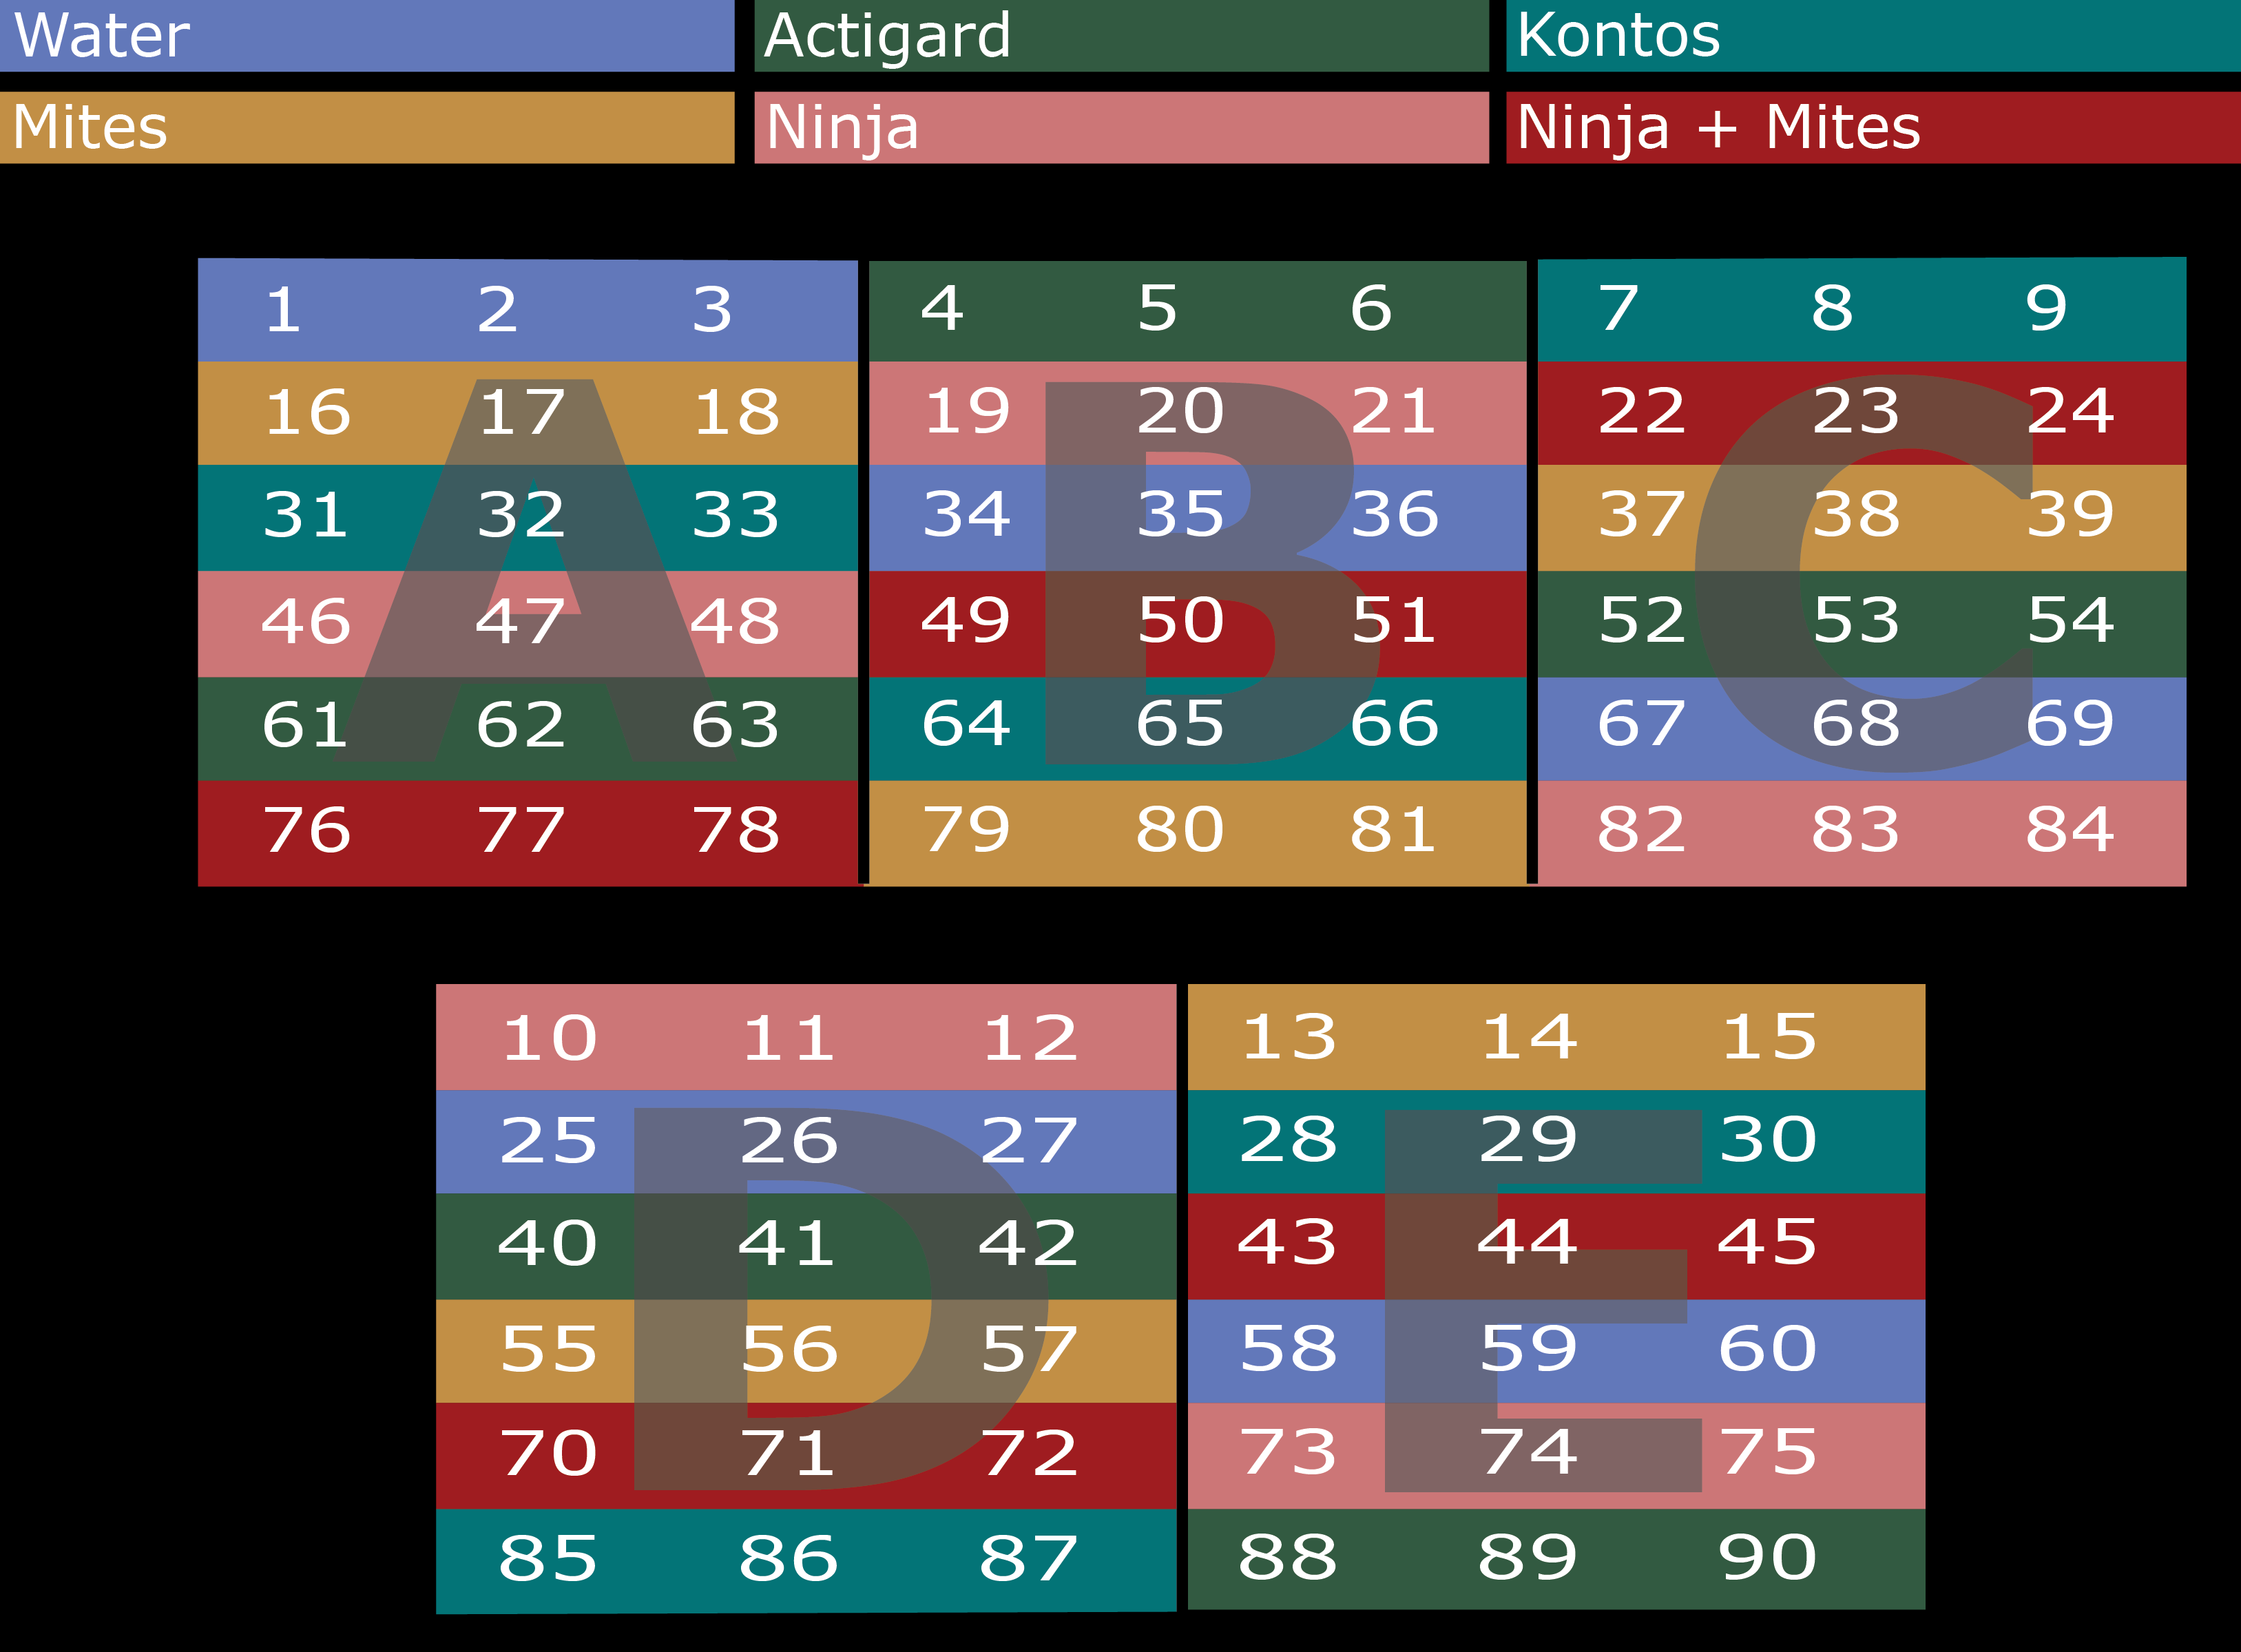
\includegraphics[width=45.19in]{figure/rrv_ipm_plot_map_2019_athens} \caption[Field design for Integrated Pest Management (IPM) trials on Pink Double Knock Out® roses to control \textit{P. fructiphilus} in Athens, GA with five treatments]{Field design for Integrated Pest Management (IPM) trials on Pink Double Knock Out® roses to control \textit{P. fructiphilus} in Athens, GA with five treatments. W = Water A = Actigard50WG, K = Kontos®, M = \textit{A. swirkii} predatory mite sachets, N = SP2700 (Trade name: Ninja, SePro), + = \textit{A. swirskii} + Ninja combined treatments. All products were applied at their label rates for 12 weeks. Flower cuttings were taken weekly to record \textit{P. fructiphilus} numbers.}\label{fig:athens-ipm-2019}
\end{figure}
\textbf{Plot Design - Griffin IPM 2019}
\begin{Shaded}
\begin{Highlighting}[]
\NormalTok{knitr}\SpecialCharTok{::}\FunctionTok{include\_graphics}\NormalTok{(}\StringTok{\textquotesingle{}figure/rrv\_ipm\_plot\_map\_2019\_griffin.png\textquotesingle{}}\NormalTok{)}
\end{Highlighting}
\end{Shaded}
\begin{figure}
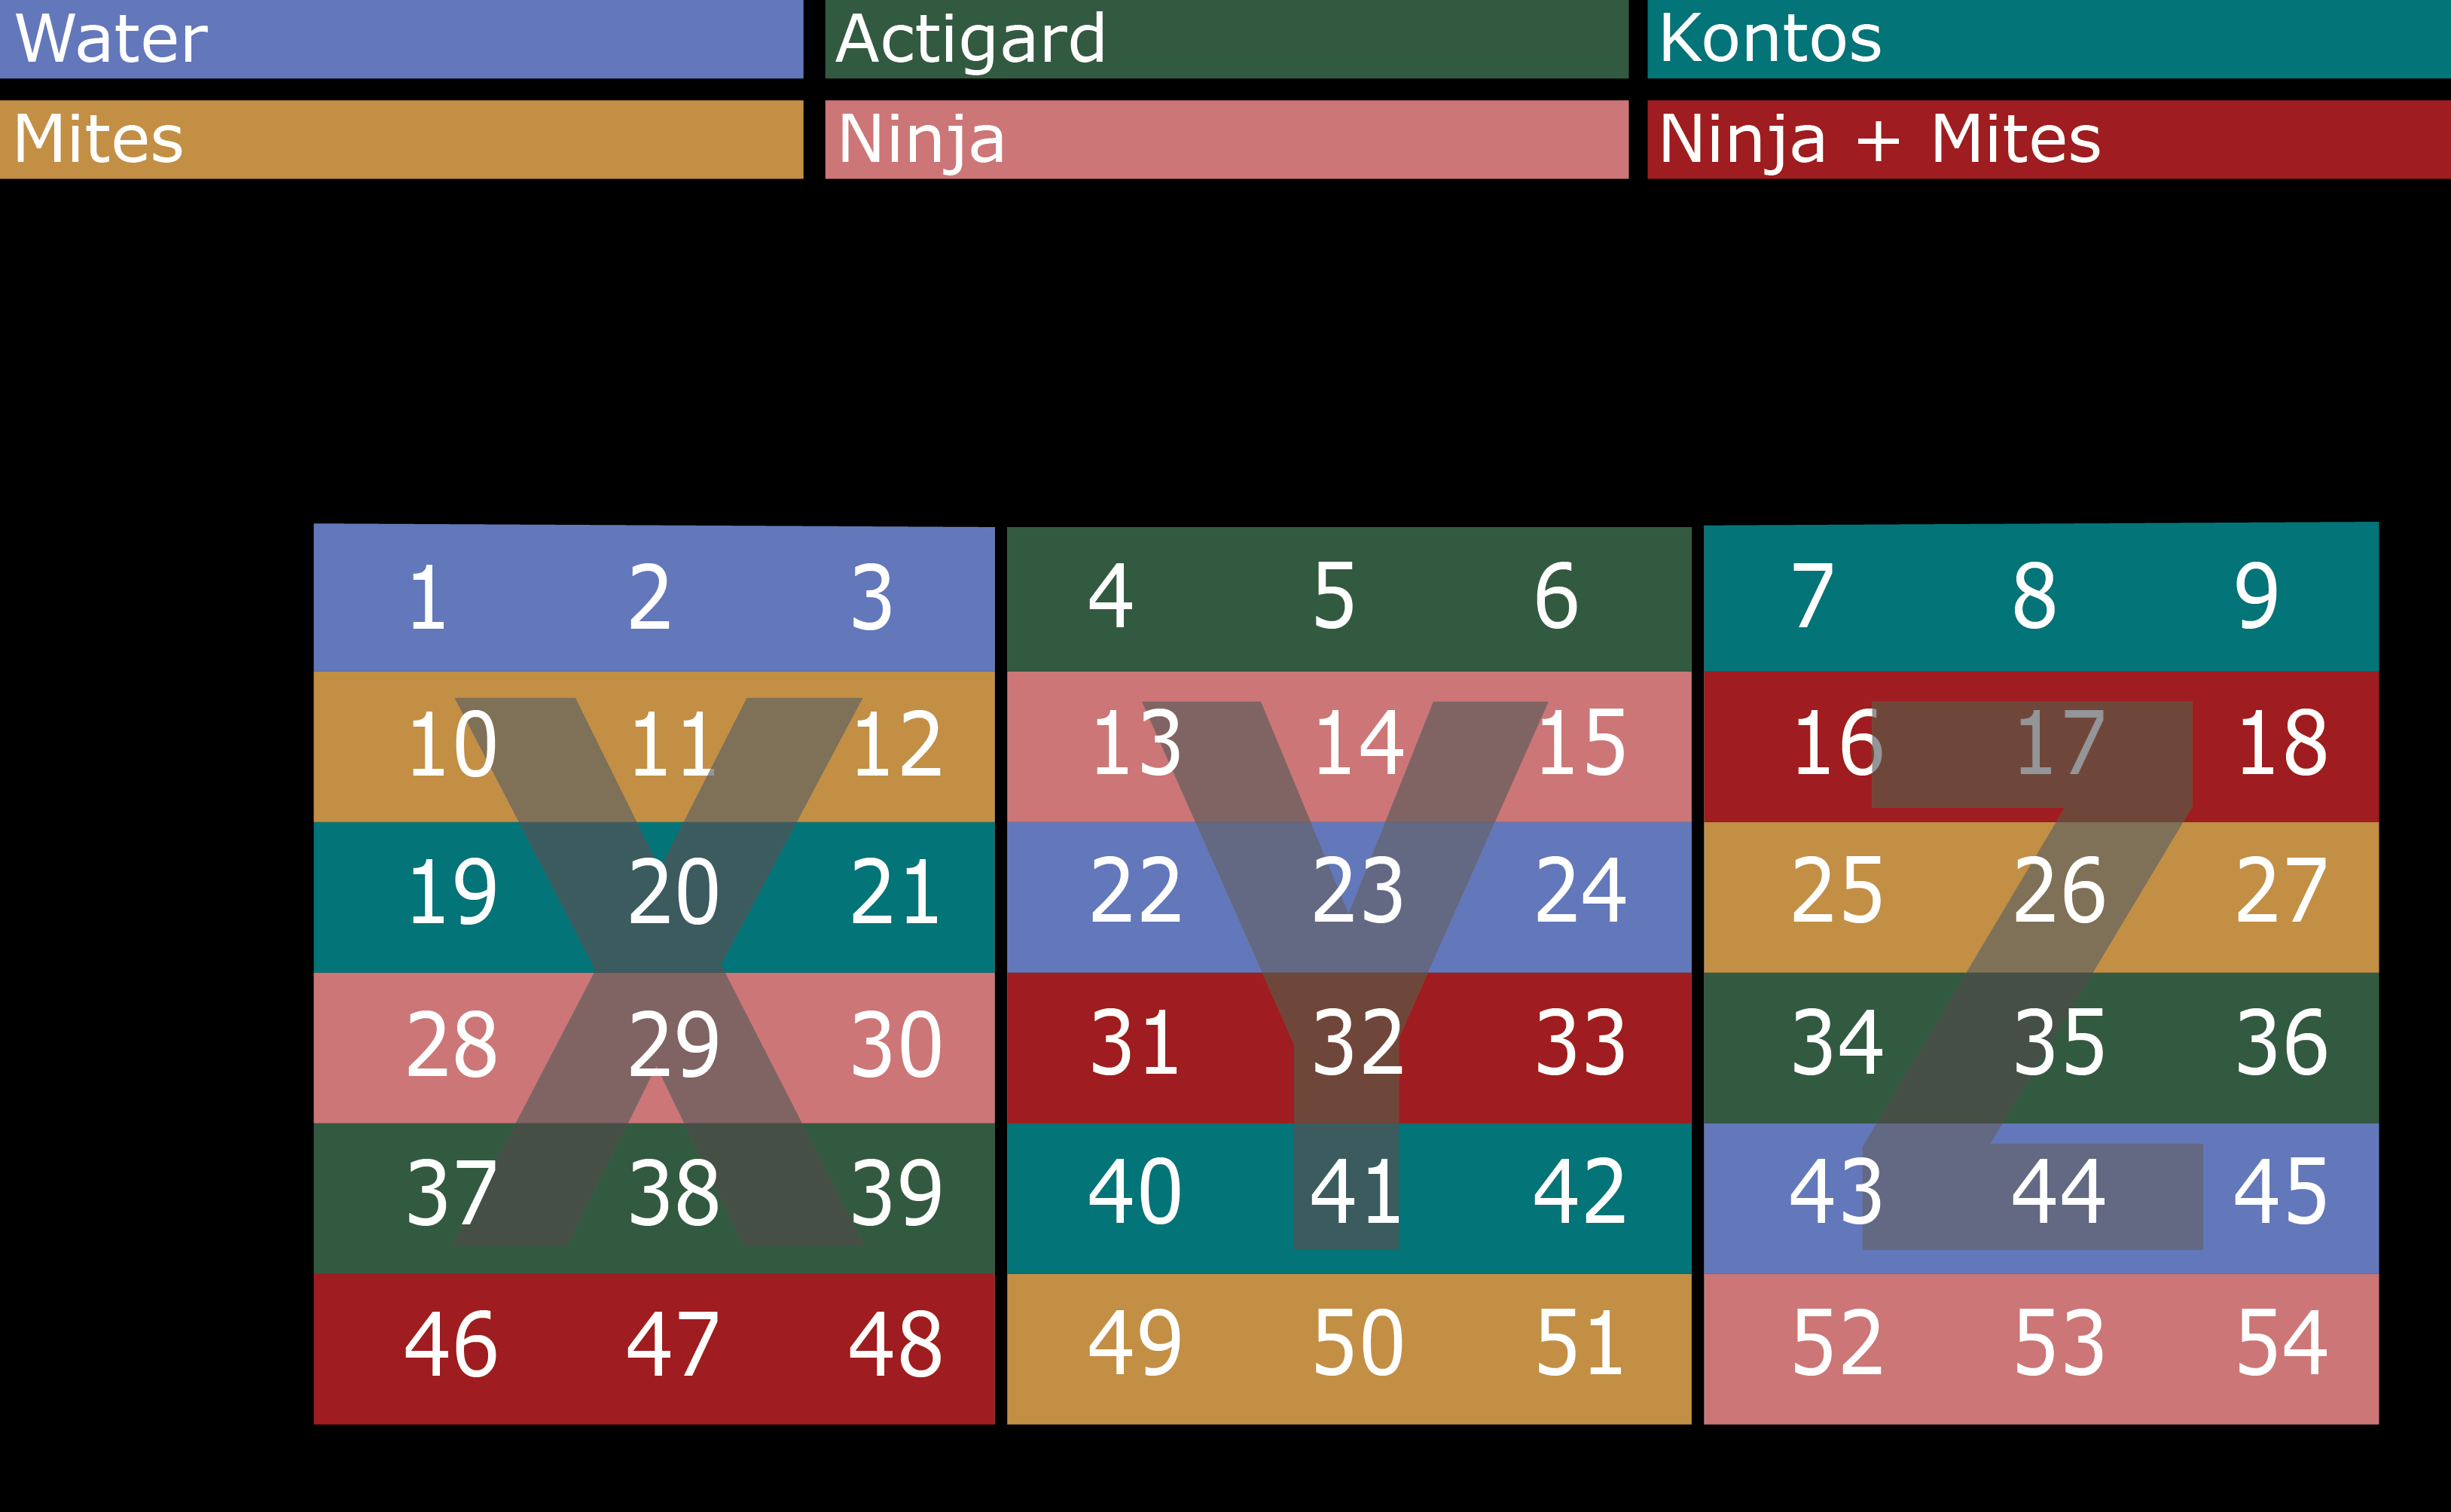
\includegraphics[width=45.19in]{figure/rrv_ipm_plot_map_2019_griffin} \caption[Field design for IPM trials on Pink Double Knock Out® roses to control \textit{P. fructiphilus} in Griffin, GA with five treatments]{Field design for IPM trials on Pink Double Knock Out® roses to control \textit{P. fructiphilus} in Griffin, GA with five treatments. W = Water A = Actigard50WG, K = Kontos®, M = \textit{A. swirkii} predatory mite sachets, N = SP2700 (Trade name: Ninja, SePro), + = \textit{A. swirskii} + Ninja combined treatments. All products were applied at their label rates for 12 weeks. Flower cuttings were taken weekly to record \textit{P. fructiphilus} numbers.}\label{fig:griff-ipm-2019}
\end{figure}
\textbf{Data Collection for Georgia IPM Trials}
Flower samples were collected from all roses once before beginning the treatments on week 1 and once at the end of the experiment on week 12. For weeks 2 through 11, flower samples were collected weekly. starting from the top rows of each block, until each row was sampled three times (see \emph{\ref{fig:athens-ipm-2019}} and \emph{\ref{fig:griff-ipm-2019}}). Disease severity was recorded weekly according to the Horsfall-Barratt Scale (\protect\hyperlink{ref-Horsfall1945}{Horsfall 1945}). Roses displaying symptoms of RRD had tissues sent to the Plant Disease Diagnostic Clinic at the North Florida Reasearch and Extension Center(PDC) for virus confirmation. Flower cuttings of about \textasciitilde12 cm were taken and placed in 50 ml centrifuge tubes. Flowers were placed flower side down and submerged with 15 ml of 95\% ethanol. Once the lid was secured, the the tube was shaken vigorously for a few seconds to help dislodge any mites. Samples were processed using the washing methods of Monfreda et al. (\protect\hyperlink{ref-Monfreda2007}{2007}), eriophyoid mites were counted and identified as previously described.

\hypertarget{phenology-field-study}{%
\subsection{Phenology field study}\label{phenology-field-study}}

In order to be sure that a further series of IPM trials would be successful, we monitored a population of \emph{P. fructiphilus} in Tallahassee which had mites but no RRD. Rose cuttings were collected periodically from four plots in the landscape of a church in Leon County, FL from 2020-2021: The site had two plantings of 2-3 years old Double Pink Knockout roses, with open sun exposure, \textasciitilde0.3 \si{\metre} spacing, and natural watering. Blocks were divided into 24 plots of \textasciitilde3 \si{\metre}\(^2\), with approximately 12 roses per plot. Samples were processed as previously described in \ref{materials-methods}. After washing, plant tissues were placed into in paper bags and put into a drying oven for \textasciitilde48 hrs at 50 °C, after which dry weight was recorded. Mites were counted and recorded to track changes in the mite populations. Roses were pruned once on the beginning of July 2020 by a professional landscaping crew.

\hypertarget{ipm-field-trials-tallahassee-2021}{%
\subsection{IPM field trials, Tallahassee 2021}\label{ipm-field-trials-tallahassee-2021}}

A second trial of IPM was conducted in Tallahassee, FL. This site did not have RRD present, but had verified populations of \emph{P. fructiphilus} present in the landscape (see APPENDIX). Spray applications were done weekly for 12 weeks from May to August 2021. Treatments were made on the same day each week, weather permitting.

\textbf{Roses}
The site was divided into two blocks, with ten plots of roses in each block. Each plot was 3 \si{m}\(^2\) with approximately 12 roses, the six roses at the center of the plot were treated, while the adjacent roses on either side was left as a buffer between plots to avoid treatment drift.

\textbf{Treatments}
Five treatments were applied: tap water as a control, Actigard50WG® (acibenzolar-S-methyl, Syngenta, Greensboro, NC, USA) - 100 \si{\milli\gram}/\si{\liter}, \emph{Amblyseius swirskii} mini sachets with hooks (Ambly-S, Arbico Organics, Oro Valley, AZ, USA) - two sachets per rose in treated plots, and a combined treatment of Actigard50WG® - 100 \si{\milli\gram}/\si{\liter} + \emph{A. swirskii} - two sachets per rose in treated plots, and a spirotetramat miticide (Kontos® Miticide Insecticide, Bayer Corporation, Whippany, New Jersey, USA), (see \emph{@(talla-ipm-2021)}).

\textbf{Mite Infestation}
\emph{P. fructiphilus} are present in the landscape of Tallahassee. Populations were present on the roses, as verified by the phenology experiments.

\textbf{Predatory mites}
The two sachets of \emph{A. swirskii} mites were applied to each of the six treated roses on the 1st, 5th and 9th week of the experiment, following the application instructions from the supplying company (Ambly-S, Arbico Organics, Oro Valley, AZ, USA). The sachets were hung from rose canes in the center of each rose. The \emph{A. swirskii} plots were also treated with water weekly when the other plots were sprayed in order to keep conditions similar to other treatments.

\textbf{Data Collection for Tallahassee IPM Trials}
Samples were collected and processed using similar methods as previously described in \ref{materials-methods}: Flower cuttings were taken weekly from from each of the six roses in the center of each plot. Three flowers (or buds if no flowers were present) were taken from each of the six central roses in each plot, for a total of 18 flowers/buds per bottle for each sampling bottle.The flowers/buds were placed into the ethanol-filled bottles and shaken vigorously for a few seconds to coat the rose tissue with ethanol and help dislodge any mites. Plant samples were processed according to the methods described in Monfreda et al. (\protect\hyperlink{ref-Monfreda2007}{2007}). Plant tissues were retained after mites were washed off, and dried in kraft paper bags and put into the oven until dry (\textasciitilde48 hrs at 50 °C), after which the dry weight of the rose tissues was recorded.
\begin{Shaded}
\begin{Highlighting}[]
\NormalTok{grid}\SpecialCharTok{::}\FunctionTok{grid.raster}\NormalTok{(tiff}\SpecialCharTok{::}\FunctionTok{readTIFF}\NormalTok{(}\StringTok{\textquotesingle{}figure/rrv\_ipm\_plot\_map\_2021\_talla.tif\textquotesingle{}}\NormalTok{))}
\end{Highlighting}
\end{Shaded}
\begin{figure}
\includegraphics{thesis_files/figure-latex/talla-ipm-2021-1} \caption[Field design for IPM trials on Pink Double Knock Out® roses to control \textit{P. fructiphilus} in Tallahassee, FL with five treatments]{Field design for IPM trials on Pink Double Knock Out® roses to control \textit{P. fructiphilus} in Tallahassee, FL with five treatments: Water, Actigard50WG®, Kontos®, \textit{Amblyseius swirkii} predatory mite sachets, and \textit{A. swirskii} + Actigard combined treatments. All products were applied at their label rates for 12 weeks. Flower cuttings were taken weekly to record \textit{P. fructiphilus} numbers.}\label{fig:talla-ipm-2021}
\end{figure}
\hypertarget{analysis-of-field-trial-data}{%
\subsection{Analysis of field trial data}\label{analysis-of-field-trial-data}}

All data from all trials was processed and analyzed using R version 4.1.1 (\protect\hyperlink{ref-RCT2021}{R Core Team 2021}). The data were all count data, so a Zero-Inflated Poisson Model (\protect\hyperlink{ref-Zeileis2008}{Zeileis et al. 2008}) was required for the ASM data (\protect\hyperlink{ref-Hothorn2008}{Hothorn et al. 2008}), while Generalized Linear Mixed Models (\protect\hyperlink{ref-Bates2015}{Bates et al. 2015}) were used for all of the IPM and phenology trials. Estimated marginal means (least squares means) (\protect\hyperlink{ref-Lenth2021}{Lenth 2021}) and Tukey Contrasts Multiple Comparisons of Means were used to determine significant effects. In addition, about \textasciitilde5\% of early samples collected from the Tallahassee field trials were missing dry weights. Missing weight data was estimated and imputted using Multivariate Imputation by Chained Equations via the mice package (\protect\hyperlink{ref-vanBuuren2011}{Buuren and Groothuis-Oudshoorn 2011}).

\hypertarget{results-2}{%
\section{Results}\label{results-2}}

\hypertarget{asm-trials}{%
\subsection{ASM trials}\label{asm-trials}}
\begin{Shaded}
\begin{Highlighting}[]
\NormalTok{knitr}\SpecialCharTok{::}\FunctionTok{include\_graphics}\NormalTok{(}\StringTok{\textquotesingle{}figure/rrv\_actigard\_graph.png\textquotesingle{}}\NormalTok{)}
\end{Highlighting}
\end{Shaded}
\begin{figure}
\includegraphics[width=66.67in]{figure/rrv_actigard_graph} \caption[SAR-induction trials on Pink Double Knock Out® roses to control \textit{Phyllocoptes fructiphilus} in Athens and Griffin, GA]{SAR-induction trials on Pink Double Knock Out® roses to control \textit{Phyllocoptes fructiphilus} in Athens and Griffin, GA. Statistical significance was determined using Tukey contrasts for multiple Comparisons of means. Groups which share letters are not statistically different from one another. $\alpha = 0.05$. water = Water Control, High = 100 \si{\milli\gram}/\si{\liter} Actigard50WG® (Syngenta, Greensboro, NC, USA) acibenzolar-S-methyl (ASM), low = 50 \si{\milli\gram}/\si{\liter} Actigard50WG® (Syngenta, Greensboro, NC, USA) acibenzolar-S-methyl (ASM), Spiro = Kontos® Miticide Insecticide - Spirotetramat (Bayer Corporation, Whippany, New Jersey, USA), All products were applied for 12 weeks. Flower cuttings were taken weekly to record the numbers of herbivorous mites.}\label{fig:asm-graph}
\end{figure}
\begin{landscape}\begin{table}

\caption{\label{tab:asm-athns-2018-table}Progression of RRD on SAR-induced Pink Double Knock Out® roses in Athens, GA 2018.}
\centering
\resizebox{\linewidth}{!}{
\begin{tabular}[t]{lrrrrrrrrrrrrrrrllrrl}
\toprule
Treatment & Block & 2018-08-31 & 2018-09-07 & 2018-09-14 & 2018-09-21 & 2018-09-28 & 2018-10-05 & 2018-10-12 & 2018-10-19 & 2018-10-26 & 2018-11-02 & 2018-12-19 & AUDPC & Final disease severity (\%) & Sample \# & Plant & RRD & P.fructiphilus & Other Mites & Field\\
\midrule
\cellcolor{gray!6}{Water} & \cellcolor{gray!6}{1} & \cellcolor{gray!6}{0} & \cellcolor{gray!6}{0} & \cellcolor{gray!6}{0} & \cellcolor{gray!6}{0.0} & \cellcolor{gray!6}{0.0} & \cellcolor{gray!6}{0.0} & \cellcolor{gray!6}{1.5} & \cellcolor{gray!6}{1.5} & \cellcolor{gray!6}{4.5} & \cellcolor{gray!6}{1.5} & \cellcolor{gray!6}{17.5} & \cellcolor{gray!6}{124.25} & \cellcolor{gray!6}{17.5} & \cellcolor{gray!6}{1} & \cellcolor{gray!6}{W1} & \cellcolor{gray!6}{S} & \cellcolor{gray!6}{2} & \cellcolor{gray!6}{0} & \cellcolor{gray!6}{Athens}\\
Water & 2 & 0 & 0 & 0 & 0.0 & 0.0 & 0.0 & 0.0 & 1.5 & 4.5 & 1.5 & 0.0 & 52.50 & 0.0 & 2 & W2 & A? & 0 & 0 & Athens\\
\cellcolor{gray!6}{Water} & \cellcolor{gray!6}{3} & \cellcolor{gray!6}{0} & \cellcolor{gray!6}{0} & \cellcolor{gray!6}{0} & \cellcolor{gray!6}{0.0} & \cellcolor{gray!6}{0.0} & \cellcolor{gray!6}{0.0} & \cellcolor{gray!6}{0.0} & \cellcolor{gray!6}{1.5} & \cellcolor{gray!6}{4.5} & \cellcolor{gray!6}{1.5} & \cellcolor{gray!6}{1.5} & \cellcolor{gray!6}{57.75} & \cellcolor{gray!6}{1.5} & \cellcolor{gray!6}{3} & \cellcolor{gray!6}{W3} & \cellcolor{gray!6}{A} & \cellcolor{gray!6}{0} & \cellcolor{gray!6}{0} & \cellcolor{gray!6}{Athens}\\
Water & 4 & 0 & 0 & 0 & 0.0 & 0.0 & 0.0 & 1.5 & 1.5 & 0.0 & 1.5 & 0.0 & 31.50 & 0.0 & 4 & W4 & A & 0 & 0 & Athens\\
\cellcolor{gray!6}{Water} & \cellcolor{gray!6}{5} & \cellcolor{gray!6}{0} & \cellcolor{gray!6}{0} & \cellcolor{gray!6}{0} & \cellcolor{gray!6}{0.0} & \cellcolor{gray!6}{0.0} & \cellcolor{gray!6}{0.0} & \cellcolor{gray!6}{1.5} & \cellcolor{gray!6}{1.5} & \cellcolor{gray!6}{0.0} & \cellcolor{gray!6}{0.0} & \cellcolor{gray!6}{9.0} & \cellcolor{gray!6}{52.50} & \cellcolor{gray!6}{9.0} & \cellcolor{gray!6}{5} & \cellcolor{gray!6}{W5} & \cellcolor{gray!6}{S} & \cellcolor{gray!6}{0} & \cellcolor{gray!6}{0} & \cellcolor{gray!6}{Athens}\\
\addlinespace
Water & 6 & 0 & 0 & 0 & 0.0 & 0.0 & 0.0 & 1.5 & 1.5 & 1.5 & 1.5 & 9.0 & 73.50 & 9.0 & 6 & W6 & S & 1 & 1 & Athens\\
\cellcolor{gray!6}{Water} & \cellcolor{gray!6}{7} & \cellcolor{gray!6}{0} & \cellcolor{gray!6}{0} & \cellcolor{gray!6}{0} & \cellcolor{gray!6}{0.0} & \cellcolor{gray!6}{0.0} & \cellcolor{gray!6}{0.0} & \cellcolor{gray!6}{0.0} & \cellcolor{gray!6}{0.0} & \cellcolor{gray!6}{1.5} & \cellcolor{gray!6}{1.5} & \cellcolor{gray!6}{1.5} & \cellcolor{gray!6}{26.25} & \cellcolor{gray!6}{1.5} & \cellcolor{gray!6}{7} & \cellcolor{gray!6}{W7} & \cellcolor{gray!6}{A} & \cellcolor{gray!6}{0} & \cellcolor{gray!6}{0} & \cellcolor{gray!6}{Athens}\\
Water & 8 & 0 & 0 & 0 & 0.0 & 0.0 & 0.0 & 0.0 & 0.0 & 1.5 & 1.5 & 4.5 & 36.75 & 4.5 & 8 & W8 & A? & 0 & 0 & Athens\\
\cellcolor{gray!6}{Water} & \cellcolor{gray!6}{9} & \cellcolor{gray!6}{0} & \cellcolor{gray!6}{0} & \cellcolor{gray!6}{0} & \cellcolor{gray!6}{0.0} & \cellcolor{gray!6}{0.0} & \cellcolor{gray!6}{0.0} & \cellcolor{gray!6}{1.5} & \cellcolor{gray!6}{1.5} & \cellcolor{gray!6}{1.5} & \cellcolor{gray!6}{1.5} & \cellcolor{gray!6}{0.0} & \cellcolor{gray!6}{42.00} & \cellcolor{gray!6}{0.0} & \cellcolor{gray!6}{9} & \cellcolor{gray!6}{W9} & \cellcolor{gray!6}{A} & \cellcolor{gray!6}{0} & \cellcolor{gray!6}{0} & \cellcolor{gray!6}{Athens}\\
Water & 10 & 0 & 0 & 0 & 0.0 & 0.0 & 0.0 & 0.0 & 1.5 & 1.5 & 1.5 & 0.0 & 31.50 & 0.0 & 10 & W10 & A? & 0 & 0 & Athens\\
\addlinespace
\cellcolor{gray!6}{Water} & \cellcolor{gray!6}{11} & \cellcolor{gray!6}{0} & \cellcolor{gray!6}{0} & \cellcolor{gray!6}{0} & \cellcolor{gray!6}{0.0} & \cellcolor{gray!6}{0.0} & \cellcolor{gray!6}{1.5} & \cellcolor{gray!6}{0.0} & \cellcolor{gray!6}{0.0} & \cellcolor{gray!6}{1.5} & \cellcolor{gray!6}{1.5} & \cellcolor{gray!6}{1.5} & \cellcolor{gray!6}{36.75} & \cellcolor{gray!6}{1.5} & \cellcolor{gray!6}{11} & \cellcolor{gray!6}{W11} & \cellcolor{gray!6}{A?} & \cellcolor{gray!6}{0} & \cellcolor{gray!6}{0} & \cellcolor{gray!6}{Athens}\\
Water & 12 & 0 & 0 & 0 & 0.0 & 0.0 & 0.0 & 1.5 & 1.5 & 1.5 & 1.5 & 17.5 & 103.25 & 17.5 & 12 & W12 & S & 0 & 1 & Athens\\
\cellcolor{gray!6}{Low} & \cellcolor{gray!6}{1} & \cellcolor{gray!6}{0} & \cellcolor{gray!6}{0} & \cellcolor{gray!6}{0} & \cellcolor{gray!6}{0.0} & \cellcolor{gray!6}{0.0} & \cellcolor{gray!6}{0.0} & \cellcolor{gray!6}{0.0} & \cellcolor{gray!6}{1.5} & \cellcolor{gray!6}{4.5} & \cellcolor{gray!6}{1.5} & \cellcolor{gray!6}{0.0} & \cellcolor{gray!6}{52.50} & \cellcolor{gray!6}{0.0} & \cellcolor{gray!6}{13} & \cellcolor{gray!6}{L1} & \cellcolor{gray!6}{A} & \cellcolor{gray!6}{0} & \cellcolor{gray!6}{0} & \cellcolor{gray!6}{Athens}\\
Low & 2 & 0 & 0 & 0 & 0.0 & 0.0 & 0.0 & 0.0 & 0.0 & 1.5 & 1.5 & 4.5 & 36.75 & 4.5 & 14 & L2 & A & 0 & 0 & Athens\\
\cellcolor{gray!6}{Low} & \cellcolor{gray!6}{3} & \cellcolor{gray!6}{0} & \cellcolor{gray!6}{0} & \cellcolor{gray!6}{0} & \cellcolor{gray!6}{0.0} & \cellcolor{gray!6}{0.0} & \cellcolor{gray!6}{0.0} & \cellcolor{gray!6}{4.5} & \cellcolor{gray!6}{1.5} & \cellcolor{gray!6}{4.5} & \cellcolor{gray!6}{0.0} & \cellcolor{gray!6}{1.5} & \cellcolor{gray!6}{78.75} & \cellcolor{gray!6}{1.5} & \cellcolor{gray!6}{15} & \cellcolor{gray!6}{L3} & \cellcolor{gray!6}{S} & \cellcolor{gray!6}{0} & \cellcolor{gray!6}{0} & \cellcolor{gray!6}{Athens}\\
\addlinespace
Low & 4 & 0 & 0 & 0 & 0.0 & 0.0 & 1.5 & 1.5 & 1.5 & 0.0 & 0.0 & 1.5 & 36.75 & 1.5 & 16 & L4 & A & 0 & 0 & Athens\\
\cellcolor{gray!6}{Low} & \cellcolor{gray!6}{5} & \cellcolor{gray!6}{0} & \cellcolor{gray!6}{0} & \cellcolor{gray!6}{0} & \cellcolor{gray!6}{0.0} & \cellcolor{gray!6}{0.0} & \cellcolor{gray!6}{1.5} & \cellcolor{gray!6}{0.0} & \cellcolor{gray!6}{1.5} & \cellcolor{gray!6}{0.0} & \cellcolor{gray!6}{0.0} & \cellcolor{gray!6}{17.5} & \cellcolor{gray!6}{82.25} & \cellcolor{gray!6}{17.5} & \cellcolor{gray!6}{17} & \cellcolor{gray!6}{L5} & \cellcolor{gray!6}{S} & \cellcolor{gray!6}{0} & \cellcolor{gray!6}{0} & \cellcolor{gray!6}{Athens}\\
Low & 6 & 0 & 0 & 0 & 0.0 & 0.0 & 0.0 & 0.0 & 0.0 & 0.0 & 1.5 & 9.0 & 42.00 & 9.0 & 18 & L6 & A & 0 & 0 & Athens\\
\cellcolor{gray!6}{Low} & \cellcolor{gray!6}{7} & \cellcolor{gray!6}{0} & \cellcolor{gray!6}{0} & \cellcolor{gray!6}{0} & \cellcolor{gray!6}{1.5} & \cellcolor{gray!6}{1.5} & \cellcolor{gray!6}{1.5} & \cellcolor{gray!6}{0.0} & \cellcolor{gray!6}{0.0} & \cellcolor{gray!6}{1.5} & \cellcolor{gray!6}{1.5} & \cellcolor{gray!6}{17.5} & \cellcolor{gray!6}{113.75} & \cellcolor{gray!6}{17.5} & \cellcolor{gray!6}{19} & \cellcolor{gray!6}{L7} & \cellcolor{gray!6}{S} & \cellcolor{gray!6}{0} & \cellcolor{gray!6}{0} & \cellcolor{gray!6}{Athens}\\
Low & 8 & 0 & 0 & 0 & 0.0 & 1.5 & 1.5 & 4.5 & 1.5 & 1.5 & 1.5 & 4.5 & 99.75 & 4.5 & 20 & L8 & A & 0 & 0 & Athens\\
\addlinespace
\cellcolor{gray!6}{Low} & \cellcolor{gray!6}{9} & \cellcolor{gray!6}{0} & \cellcolor{gray!6}{0} & \cellcolor{gray!6}{0} & \cellcolor{gray!6}{0.0} & \cellcolor{gray!6}{0.0} & \cellcolor{gray!6}{0.0} & \cellcolor{gray!6}{1.5} & \cellcolor{gray!6}{0.0} & \cellcolor{gray!6}{0.0} & \cellcolor{gray!6}{0.0} & \cellcolor{gray!6}{17.5} & \cellcolor{gray!6}{71.75} & \cellcolor{gray!6}{17.5} & \cellcolor{gray!6}{21} & \cellcolor{gray!6}{L9} & \cellcolor{gray!6}{S} & \cellcolor{gray!6}{0} & \cellcolor{gray!6}{0} & \cellcolor{gray!6}{Athens}\\
Low & 10 & 0 & 0 & 0 & 0.0 & 0.0 & 0.0 & 1.5 & 1.5 & 0.0 & 1.5 & 4.5 & 47.25 & 4.5 & 22 & L10 & A & 0 & 0 & Athens\\
\cellcolor{gray!6}{Low} & \cellcolor{gray!6}{11} & \cellcolor{gray!6}{0} & \cellcolor{gray!6}{0} & \cellcolor{gray!6}{0} & \cellcolor{gray!6}{0.0} & \cellcolor{gray!6}{0.0} & \cellcolor{gray!6}{0.0} & \cellcolor{gray!6}{0.0} & \cellcolor{gray!6}{1.5} & \cellcolor{gray!6}{4.5} & \cellcolor{gray!6}{1.5} & \cellcolor{gray!6}{0.0} & \cellcolor{gray!6}{52.50} & \cellcolor{gray!6}{0.0} & \cellcolor{gray!6}{23} & \cellcolor{gray!6}{L11} & \cellcolor{gray!6}{A} & \cellcolor{gray!6}{0} & \cellcolor{gray!6}{0} & \cellcolor{gray!6}{Athens}\\
Low & 12 & 0 & 0 & 0 & 0.0 & 0.0 & 1.5 & 0.0 & 0.0 & 1.5 & 1.5 & 1.5 & 36.75 & 1.5 & 24 & L12 & A & 0 & 0 & Athens\\
\cellcolor{gray!6}{High} & \cellcolor{gray!6}{1} & \cellcolor{gray!6}{0} & \cellcolor{gray!6}{0} & \cellcolor{gray!6}{0} & \cellcolor{gray!6}{0.0} & \cellcolor{gray!6}{0.0} & \cellcolor{gray!6}{0.0} & \cellcolor{gray!6}{1.5} & \cellcolor{gray!6}{0.0} & \cellcolor{gray!6}{4.5} & \cellcolor{gray!6}{4.5} & \cellcolor{gray!6}{1.5} & \cellcolor{gray!6}{78.75} & \cellcolor{gray!6}{1.5} & \cellcolor{gray!6}{25} & \cellcolor{gray!6}{H1} & \cellcolor{gray!6}{S?} & \cellcolor{gray!6}{0} & \cellcolor{gray!6}{0} & \cellcolor{gray!6}{Athens}\\
\addlinespace
High & 2 & 0 & 0 & 0 & 0.0 & 0.0 & 1.5 & 0.0 & 0.0 & 0.0 & 0.0 & 17.5 & 71.75 & 17.5 & 26 & H2 & S & 0 & 0 & Athens\\
\cellcolor{gray!6}{High} & \cellcolor{gray!6}{3} & \cellcolor{gray!6}{0} & \cellcolor{gray!6}{0} & \cellcolor{gray!6}{0} & \cellcolor{gray!6}{0.0} & \cellcolor{gray!6}{0.0} & \cellcolor{gray!6}{0.0} & \cellcolor{gray!6}{1.5} & \cellcolor{gray!6}{1.5} & \cellcolor{gray!6}{1.5} & \cellcolor{gray!6}{1.5} & \cellcolor{gray!6}{17.5} & \cellcolor{gray!6}{103.25} & \cellcolor{gray!6}{17.5} & \cellcolor{gray!6}{27} & \cellcolor{gray!6}{H3} & \cellcolor{gray!6}{S} & \cellcolor{gray!6}{0} & \cellcolor{gray!6}{0} & \cellcolor{gray!6}{Athens}\\
High & 4 & 0 & 0 & 0 & 0.0 & 0.0 & 0.0 & 0.0 & 0.0 & 1.5 & 1.5 & 1.5 & 26.25 & 1.5 & 28 & H4 & A & 0 & 0 & Athens\\
\cellcolor{gray!6}{High} & \cellcolor{gray!6}{5} & \cellcolor{gray!6}{0} & \cellcolor{gray!6}{0} & \cellcolor{gray!6}{0} & \cellcolor{gray!6}{0.0} & \cellcolor{gray!6}{0.0} & \cellcolor{gray!6}{0.0} & \cellcolor{gray!6}{0.0} & \cellcolor{gray!6}{1.5} & \cellcolor{gray!6}{1.5} & \cellcolor{gray!6}{1.5} & \cellcolor{gray!6}{4.5} & \cellcolor{gray!6}{47.25} & \cellcolor{gray!6}{4.5} & \cellcolor{gray!6}{29} & \cellcolor{gray!6}{H5} & \cellcolor{gray!6}{S} & \cellcolor{gray!6}{0} & \cellcolor{gray!6}{0} & \cellcolor{gray!6}{Athens}\\
High & 6 & 0 & 0 & 0 & 0.0 & 0.0 & 0.0 & 0.0 & 1.5 & 1.5 & 1.5 & 0.0 & 31.50 & 0.0 & 30 & H6 & A & 0 & 0 & Athens\\
\addlinespace
\cellcolor{gray!6}{High} & \cellcolor{gray!6}{7} & \cellcolor{gray!6}{0} & \cellcolor{gray!6}{0} & \cellcolor{gray!6}{0} & \cellcolor{gray!6}{0.0} & \cellcolor{gray!6}{0.0} & \cellcolor{gray!6}{0.0} & \cellcolor{gray!6}{0.0} & \cellcolor{gray!6}{0.0} & \cellcolor{gray!6}{0.0} & \cellcolor{gray!6}{1.5} & \cellcolor{gray!6}{4.5} & \cellcolor{gray!6}{26.25} & \cellcolor{gray!6}{4.5} & \cellcolor{gray!6}{31} & \cellcolor{gray!6}{H7} & \cellcolor{gray!6}{S} & \cellcolor{gray!6}{0} & \cellcolor{gray!6}{0} & \cellcolor{gray!6}{Athens}\\
High & 8 & 0 & 0 & 0 & 1.5 & 1.5 & 1.5 & 1.5 & 1.5 & 4.5 & 4.5 & 62.5 & 334.25 & 62.5 & 32 & H8 & S & 1 & 0 & Athens\\
\cellcolor{gray!6}{High} & \cellcolor{gray!6}{9} & \cellcolor{gray!6}{0} & \cellcolor{gray!6}{0} & \cellcolor{gray!6}{0} & \cellcolor{gray!6}{0.0} & \cellcolor{gray!6}{0.0} & \cellcolor{gray!6}{0.0} & \cellcolor{gray!6}{1.5} & \cellcolor{gray!6}{1.5} & \cellcolor{gray!6}{1.5} & \cellcolor{gray!6}{1.5} & \cellcolor{gray!6}{17.5} & \cellcolor{gray!6}{103.25} & \cellcolor{gray!6}{17.5} & \cellcolor{gray!6}{33} & \cellcolor{gray!6}{H9} & \cellcolor{gray!6}{S} & \cellcolor{gray!6}{0} & \cellcolor{gray!6}{0} & \cellcolor{gray!6}{Athens}\\
High & 10 & 0 & 0 & 0 & 0.0 & 0.0 & 1.5 & 1.5 & 0.0 & 1.5 & 1.5 & 0.0 & 42.00 & 0.0 & 34 & H10 & A & 0 & 0 & Athens\\
\cellcolor{gray!6}{High} & \cellcolor{gray!6}{11} & \cellcolor{gray!6}{0} & \cellcolor{gray!6}{0} & \cellcolor{gray!6}{0} & \cellcolor{gray!6}{0.0} & \cellcolor{gray!6}{0.0} & \cellcolor{gray!6}{0.0} & \cellcolor{gray!6}{0.0} & \cellcolor{gray!6}{0.0} & \cellcolor{gray!6}{0.0} & \cellcolor{gray!6}{0.0} & \cellcolor{gray!6}{1.5} & \cellcolor{gray!6}{5.25} & \cellcolor{gray!6}{1.5} & \cellcolor{gray!6}{35} & \cellcolor{gray!6}{H11} & \cellcolor{gray!6}{A} & \cellcolor{gray!6}{0} & \cellcolor{gray!6}{0} & \cellcolor{gray!6}{Athens}\\
\addlinespace
High & 12 & 0 & 0 & 0 & 0.0 & 0.0 & 1.5 & 0.0 & 0.0 & 0.0 & 0.0 & 0.0 & 10.50 & 0.0 & 36 & H12 & A & 0 & 0 & Athens\\
\cellcolor{gray!6}{NoTrt} & \cellcolor{gray!6}{1} & \cellcolor{gray!6}{0} & \cellcolor{gray!6}{0} & \cellcolor{gray!6}{0} & \cellcolor{gray!6}{0.0} & \cellcolor{gray!6}{0.0} & \cellcolor{gray!6}{0.0} & \cellcolor{gray!6}{0.0} & \cellcolor{gray!6}{0.0} & \cellcolor{gray!6}{0.0} & \cellcolor{gray!6}{0.0} & \cellcolor{gray!6}{0.0} & \cellcolor{gray!6}{0.00} & \cellcolor{gray!6}{0.0} & \cellcolor{gray!6}{37} & \cellcolor{gray!6}{C1} & \cellcolor{gray!6}{A} & \cellcolor{gray!6}{0} & \cellcolor{gray!6}{0} & \cellcolor{gray!6}{Athens}\\
NoTrt & 2 & 0 & 0 & 0 & 0.0 & 0.0 & 0.0 & 0.0 & 0.0 & 0.0 & 0.0 & 1.5 & 5.25 & 1.5 & 38 & C2 & A & 0 & 0 & Athens\\
\cellcolor{gray!6}{NoTrt} & \cellcolor{gray!6}{3} & \cellcolor{gray!6}{0} & \cellcolor{gray!6}{0} & \cellcolor{gray!6}{0} & \cellcolor{gray!6}{0.0} & \cellcolor{gray!6}{0.0} & \cellcolor{gray!6}{0.0} & \cellcolor{gray!6}{0.0} & \cellcolor{gray!6}{0.0} & \cellcolor{gray!6}{0.0} & \cellcolor{gray!6}{0.0} & \cellcolor{gray!6}{0.0} & \cellcolor{gray!6}{0.00} & \cellcolor{gray!6}{0.0} & \cellcolor{gray!6}{39} & \cellcolor{gray!6}{C3} & \cellcolor{gray!6}{A} & \cellcolor{gray!6}{0} & \cellcolor{gray!6}{0} & \cellcolor{gray!6}{Athens}\\
NoTrt & 4 & 0 & 0 & 0 & 0.0 & 0.0 & 0.0 & 0.0 & 0.0 & 0.0 & 0.0 & 1.5 & 5.25 & 1.5 & 40 & C4 & A & 0 & 0 & Athens\\
\addlinespace
\cellcolor{gray!6}{NoTrt} & \cellcolor{gray!6}{5} & \cellcolor{gray!6}{0} & \cellcolor{gray!6}{0} & \cellcolor{gray!6}{0} & \cellcolor{gray!6}{0.0} & \cellcolor{gray!6}{0.0} & \cellcolor{gray!6}{0.0} & \cellcolor{gray!6}{0.0} & \cellcolor{gray!6}{0.0} & \cellcolor{gray!6}{0.0} & \cellcolor{gray!6}{0.0} & \cellcolor{gray!6}{0.0} & \cellcolor{gray!6}{0.00} & \cellcolor{gray!6}{0.0} & \cellcolor{gray!6}{41} & \cellcolor{gray!6}{C5} & \cellcolor{gray!6}{A} & \cellcolor{gray!6}{0} & \cellcolor{gray!6}{0} & \cellcolor{gray!6}{Athens}\\
NoTrt & 6 & 0 & 0 & 0 & 0.0 & 0.0 & 0.0 & 0.0 & 0.0 & 0.0 & 0.0 & 0.0 & 0.00 & 0.0 & 42 & C6 & A & 0 & 0 & Athens\\
\cellcolor{gray!6}{NoTrt} & \cellcolor{gray!6}{7} & \cellcolor{gray!6}{0} & \cellcolor{gray!6}{0} & \cellcolor{gray!6}{0} & \cellcolor{gray!6}{0.0} & \cellcolor{gray!6}{0.0} & \cellcolor{gray!6}{0.0} & \cellcolor{gray!6}{0.0} & \cellcolor{gray!6}{0.0} & \cellcolor{gray!6}{0.0} & \cellcolor{gray!6}{0.0} & \cellcolor{gray!6}{0.0} & \cellcolor{gray!6}{0.00} & \cellcolor{gray!6}{0.0} & \cellcolor{gray!6}{43} & \cellcolor{gray!6}{C7} & \cellcolor{gray!6}{A} & \cellcolor{gray!6}{0} & \cellcolor{gray!6}{0} & \cellcolor{gray!6}{Athens}\\
NoTrt & 8 & 0 & 0 & 0 & 0.0 & 0.0 & 0.0 & 0.0 & 0.0 & 0.0 & 0.0 & 0.0 & 0.00 & 0.0 & 44 & C8 & A & 0 & 0 & Athens\\
\cellcolor{gray!6}{NoTrt} & \cellcolor{gray!6}{9} & \cellcolor{gray!6}{0} & \cellcolor{gray!6}{0} & \cellcolor{gray!6}{0} & \cellcolor{gray!6}{0.0} & \cellcolor{gray!6}{0.0} & \cellcolor{gray!6}{0.0} & \cellcolor{gray!6}{0.0} & \cellcolor{gray!6}{0.0} & \cellcolor{gray!6}{0.0} & \cellcolor{gray!6}{0.0} & \cellcolor{gray!6}{0.0} & \cellcolor{gray!6}{0.00} & \cellcolor{gray!6}{0.0} & \cellcolor{gray!6}{45} & \cellcolor{gray!6}{C9} & \cellcolor{gray!6}{A} & \cellcolor{gray!6}{0} & \cellcolor{gray!6}{0} & \cellcolor{gray!6}{Athens}\\
\addlinespace
NoTrt & 10 & 0 & 0 & 0 & 0.0 & 0.0 & 0.0 & 0.0 & 0.0 & 0.0 & 0.0 & 1.5 & 5.25 & 1.5 & 46 & C10 & A & 0 & 0 & Athens\\
\cellcolor{gray!6}{NoTrt} & \cellcolor{gray!6}{11} & \cellcolor{gray!6}{0} & \cellcolor{gray!6}{0} & \cellcolor{gray!6}{0} & \cellcolor{gray!6}{0.0} & \cellcolor{gray!6}{0.0} & \cellcolor{gray!6}{0.0} & \cellcolor{gray!6}{0.0} & \cellcolor{gray!6}{0.0} & \cellcolor{gray!6}{0.0} & \cellcolor{gray!6}{0.0} & \cellcolor{gray!6}{0.0} & \cellcolor{gray!6}{0.00} & \cellcolor{gray!6}{0.0} & \cellcolor{gray!6}{47} & \cellcolor{gray!6}{C11} & \cellcolor{gray!6}{A} & \cellcolor{gray!6}{0} & \cellcolor{gray!6}{0} & \cellcolor{gray!6}{Athens}\\
NoTrt & 12 & 0 & 0 & 0 & 0.0 & 0.0 & 0.0 & 0.0 & 0.0 & 0.0 & 0.0 & 0.0 & 0.00 & 0.0 & 48 & C12 & A & 0 & 0 & Athens\\
\bottomrule
\end{tabular}}
\end{table}
\end{landscape}
\hypertarget{phenology}{%
\subsection{Phenology}\label{phenology}}
\begin{Shaded}
\begin{Highlighting}[]
\NormalTok{knitr}\SpecialCharTok{::}\FunctionTok{include\_graphics}\NormalTok{(}\StringTok{\textquotesingle{}figure/rrv\_pheno\_bargraph.png\textquotesingle{}}\NormalTok{)}
\end{Highlighting}
\end{Shaded}
\begin{figure}[h]
\includegraphics[width=66.67in]{figure/rrv_pheno_bargraph} \caption[Phenology of \textit{P. fructiphilus} mite populations on roses in Leon County, Florida]{Phenology of \textit{P. fructiphilus} mite populations on roses in Leon County, Florida 2020-2021. Roses were pruned back heavily on July 9, 2020.}\label{fig:pheno-graphs}
\end{figure}
\hypertarget{ipm-trials}{%
\subsection{IPM trials}\label{ipm-trials}}
\begin{Shaded}
\begin{Highlighting}[]
\NormalTok{knitr}\SpecialCharTok{::}\FunctionTok{include\_graphics}\NormalTok{(}\StringTok{\textquotesingle{}figure/rrv\_ipm\_graph\_erios\_talla.png\textquotesingle{}}\NormalTok{)}
\end{Highlighting}
\end{Shaded}
\begin{figure}
\includegraphics[width=66.67in]{figure/rrv_ipm_graph_erios_talla} \caption[IPM trials on Pink Double Knock Out® roses to control \textit{P. fructiphilus} in Tallahassee, FL with five treatments]{IPM trials on Pink Double Knock Out® roses to control \textit{P. fructiphilus} in Tallahassee, FL with five treatments. Statistical significance was determined using Tukey contrasts for multiple Comparisons of means. Groups which share letters are not statistically different from one another. $\alpha = 0.05$. Water = Water Control, ASM = Actigard50WG® (Syngenta, Greensboro, NC, USA) acibenzolar-S-methyl (ASM), Spiro = Kontos® Miticide Insecticide - Spirotetramat (Bayer Corporation, Whippany, New Jersey, USA), Mites = \textit{Amblyseius swirkii} predatory mite mini sachets on hooks (Ambly-S, Arbico Organics, Oro Valley, AZ, USA), MA = \textit{A. swirskii} + Actigard combined treatments. All products were applied at their label rates for 12 weeks. Flower cuttings were taken weekly to record the numbers of \textit{P. fructiphilus} and other herbivorous mites.}\label{fig:ipm-talla-erios}
\end{figure}
\begin{Shaded}
\begin{Highlighting}[]
\NormalTok{knitr}\SpecialCharTok{::}\FunctionTok{include\_graphics}\NormalTok{(}\StringTok{\textquotesingle{}figure/rrv\_ipm\_graph\_erios\_talla\_month.png\textquotesingle{}}\NormalTok{)}
\end{Highlighting}
\end{Shaded}
\begin{figure}
\includegraphics[width=66.67in]{figure/rrv_ipm_graph_erios_talla_month} \caption{IPM trials on Pink Double Knock Out® roses to control \textit{P. fructiphilus} in Tallahassee, FL with five treatments}\label{fig:ipm-talla-erios-month}
\end{figure}
\begin{Shaded}
\begin{Highlighting}[]
\NormalTok{knitr}\SpecialCharTok{::}\FunctionTok{include\_graphics}\NormalTok{(}\StringTok{\textquotesingle{}figure/rrv\_ipm\_graph\_tets\_talla.png\textquotesingle{}}\NormalTok{)}
\end{Highlighting}
\end{Shaded}
\begin{figure}
\includegraphics[width=66.67in]{figure/rrv_ipm_graph_tets_talla} \caption{IPM trials on Pink Double Knock Out® roses to control \textit{P. fructiphilus} in Tallahassee, FL with five treatments}\label{fig:ipm-talla-tets}
\end{figure}
\begin{Shaded}
\begin{Highlighting}[]
\NormalTok{knitr}\SpecialCharTok{::}\FunctionTok{include\_graphics}\NormalTok{(}\StringTok{\textquotesingle{}figure/rrv\_ipm\_graph\_tets\_talla\_month.png\textquotesingle{}}\NormalTok{)}
\end{Highlighting}
\end{Shaded}
\begin{figure}
\includegraphics[width=66.67in]{figure/rrv_ipm_graph_tets_talla_month} \caption{IPM trials on Pink Double Knock Out® roses to control \textit{P. fructiphilus} in Tallahassee, FL with five treatments}\label{fig:ipm-talla-tets-month}
\end{figure}
\begin{Shaded}
\begin{Highlighting}[]
\NormalTok{knitr}\SpecialCharTok{::}\FunctionTok{include\_graphics}\NormalTok{(}\StringTok{\textquotesingle{}figure/rrv\_ipm\_graph\_preds\_talla.png\textquotesingle{}}\NormalTok{)}
\end{Highlighting}
\end{Shaded}
\begin{figure}
\includegraphics[width=66.67in]{figure/rrv_ipm_graph_preds_talla} \caption{IPM trials on Pink Double Knock Out® roses to control \textit{P. fructiphilus} in Tallahassee, FL with five treatments}\label{fig:ipm-talla-preds}
\end{figure}
\begin{Shaded}
\begin{Highlighting}[]
\NormalTok{knitr}\SpecialCharTok{::}\FunctionTok{include\_graphics}\NormalTok{(}\StringTok{\textquotesingle{}figure/rrv\_ipm\_graph\_preds\_talla\_month.png\textquotesingle{}}\NormalTok{)}
\end{Highlighting}
\end{Shaded}
\begin{figure}
\includegraphics[width=66.67in]{figure/rrv_ipm_graph_preds_talla_month} \caption{IPM trials on Pink Double Knock Out® roses to control \textit{P. fructiphilus} in Tallahassee, FL with five treatments}\label{fig:ipm-talla-preds-month}
\end{figure}
\hypertarget{discussion-2}{%
\section{Discussion}\label{discussion-2}}

We had low recovery of \emph{P. fructiphilus} for the ASM and IPM trials in Georgia. This lead us to the phenology study, to ensure that there had been adequate establishment of \emph{P. fructiphilus} to create measurable effects. The phenology study was successful in measuring population fluctuations of eriophyid mites, and helped guarantee the presence of \emph{P. fructiphilus} before beginning the IPM trials in Tallahassee. Our results from the the IPM trials in Tallahassee suggest that spirotetramat were able to significantly reduce populations of \emph{P. fructiphilus}, an effect seen in all of the field trials conducted. Numbers of \emph{P. fructiphilius} on ASM-treated plants were were not significantly different than the number of eriophyids on the control, even when combined with predatory mite releases (see \emph{\ref{fig:ipm-talla-erios}}). \emph{A. swirskii} were recovered in smaller numbers than the other species of mites (see \emph{\ref{fig:ipm-talla-preds}}).
Although we did not create barriers to prevent dispersal of \emph{A. swirskii}, these mites were most frequently recovered from the same plots where they were released. It is possible that we encountered few \emph{A. swirskii} because they dispersed to the point of leaving the rose plots (\protect\hyperlink{ref-Addesso2018}{Addesso et al. 2018}). This would make sense in the light of other studies: Buitenhuis et al. (\protect\hyperlink{ref-Buitenhuis2013}{2013}) noted the ability of \emph{A. swirskii} to move quickly on roses due to fewer trichomes, and recommended adjusting their release rates accordingly to maintain high populations on plants. \emph{A. swirskii} are not expected to disperse very far off of plants, but canopy connectivity between plants has been noted to increase their dispersal (\protect\hyperlink{ref-Buitenhuis2010}{Buitenhuis et al. 2010}). Ornamentals such as roses tend to be grown in separately spaced pots. Although the roses at our site were planted in the ground, the plots we tested did not have overlapping canopies, which may have reduced dispersal of \emph{A. swirskii} into other nearby roses. We anticipated seeing lower numbers of \emph{T. urticae} in plots where \emph{A. swirskii} had been released, but we did not see any correlations between releases of \emph{A. swirskii} on \emph{T. urticae}. Other studies have found \emph{A. swirskii} predation to be negatively correlated with trichome density (\protect\hyperlink{ref-Buitenhuis2013}{Buitenhuis et al. 2013}), suggesting that \emph{A. swirskii} are unlikely to feed on \emph{P. fructiphilus} hidden in the tightly appressed surfaces between rose sepals and petals. These areas also contain dense glandular trichomes, which tend to accumulate high quantities of VOCs (\protect\hyperlink{ref-Tissier2017}{Tissier et al. 2017}), defensive compounds (\protect\hyperlink{ref-Gerhold1984}{Gerhold et al. 1984}, \protect\hyperlink{ref-Ambrosio2008}{Ambrósio et al. 2008}, \protect\hyperlink{ref-Karabourniotis2019}{Karabourniotis et al. 2019}), or possibly entrap predators (\protect\hyperlink{ref-Nihoul1994}{Nihoul 1994}), benefits which erinea-producing eriophyids readily exploit to protect themselves (\protect\hyperlink{ref-Karioti2011}{Karioti et al. 2011}, \protect\hyperlink{ref-Karabourniotis2019}{Karabourniotis et al. 2019}). We did not see any correlations between \emph{A. swirskii} and \emph{P. fructiphilus}, as anticipated. Spirotetramat is known to less toxic to \emph{A. swirskii} (\protect\hyperlink{ref-Fernandez2017}{Fernández et al. 2017}), but no correlations emerged for \emph{A. swirskii} for either spirotetramat or ASM treatments. Some evidence has been given that slow release mite sachets which are sheltered and provided with felt patches (\protect\hyperlink{ref-Shimoda2017}{Shimoda et al. 2017}), and/or moisture in the form of water-absorbant sodium polyacrylate gels had better releases of predators (\protect\hyperlink{ref-Shimoda2018}{Shimoda et al. 2018}). It is also possible that there was an excess of pollen or other acceptable food sources which \emph{A. swirskii} preferred over the \emph{T. urticae} found in roses (\protect\hyperlink{ref-Leman2014}{Leman and Messelink 2014}), or competition with other predators encountered on the roses (\protect\hyperlink{ref-Doeker2021}{Döker et al. 2021}). A cursory examination of non-mite arthropods in rose samples revealed a number of unidentified species of thrips. \emph{A. swirskii} are known to feed on thrips, so there may be correlations between the predatory mites and the number of thrips in each treatment, but this requires a reexamination of the bycatch data. Populations of \emph{P. fructiphilius} showed seasonal fluctuations in mite numbers, with highest populations achieved during June 2020 and July 2021. Rose pruning in July 2020 reduced the numbers of \emph{P, fructiphilus} collected for 3 months, populations began to recover that November. However, the number of \emph{P.fructiphilus} collected was not significantly different between the years 2020 and 2021 for the phenology trials. Mite numbers remained relatively lower during 2021 compared to the previous year. None of the mite-infested roses have shown symptoms of RRD to date. Tracking populations for longer periods of time with additional climatic data could be used to determine the best times to prune and apply chemistry to reduce mite numbers. The large reductions of \emph{P. fructiphilus} seen post pruning suggests its potential as a method of cultural mite control. The combination of pruning with acaricide treatments has been previously tested to control \emph{P. fructiphilus}, with limited success (\protect\hyperlink{ref-Windham2014}{Windham et al. 2014}), but these studies were conducted in areas of high pest pressure, with the presence of RRD. It is unlikely that acaricides or pruning are sufficient to prevent RRD infection: pruning does not remove the virus (\protect\hyperlink{ref-Bello2017}{Di Bello et al. 2017}), and the inoculation access period for transmission of RRD is surprisingly short, with mites able to transmit the virus within an hour of plant feeding (\protect\hyperlink{ref-Bello2017}{Di Bello et al. 2017}). Even so, the efficacy of combining pruning and acaricides has not been tested in areas with recent introductions of the mite without the virus. Combined management treatments may prove more effective in maintaining low populations of non-viruliferious \emph{P. fruciphilus}, and should be investigated for preventing the spread of the mite, rather than preventing the disease proper.

\hypertarget{brevipalpus-transmitted-orchid-fleck-dichorhavirus-infecting-three-new-ornamental-hosts-in-florida}{%
\chapter{\texorpdfstring{\emph{Brevipalpus}-TRANSMITTED \emph{Orchid fleck dichorhavirus} INFECTING THREE NEW ORNAMENTAL HOSTS IN FLORIDA}{Brevipalpus-TRANSMITTED Orchid fleck dichorhavirus INFECTING THREE NEW ORNAMENTAL HOSTS IN FLORIDA}}\label{brevipalpus-transmitted-orchid-fleck-dichorhavirus-infecting-three-new-ornamental-hosts-in-florida}}

Placeholder

\hypertarget{virus-detection}{%
\section{Virus Detection}\label{virus-detection}}

\hypertarget{a-comment-on-the-status-of-brevipalpus-in-florida}{%
\section{\texorpdfstring{A Comment on the Status of \emph{Brevipalpus} in Florida}{A Comment on the Status of Brevipalpus in Florida}}\label{a-comment-on-the-status-of-brevipalpus-in-florida}}

\hypertarget{conclusions-invasive-mites-are-an-increasingly-large-problem-for-florida}{%
\chapter{CONCLUSIONS: INVASIVE MITES ARE AN INCREASINGLY LARGE PROBLEM FOR FLORIDA}\label{conclusions-invasive-mites-are-an-increasingly-large-problem-for-florida}}

\hypertarget{invasive-species-continue-to-be-a-problem}{%
\section{Invasive Species Continue to be a Problem}\label{invasive-species-continue-to-be-a-problem}}

The aim of our research was to address the emerging problems caused by the recent invasions of mites and the plant viruses they vector to northern Florida. Florida is a hotspot for invasive species in the mainland US, due to a combination of its unique geography, climate, rapid development and a multitude of invasion pathways (\protect\hyperlink{ref-Simberloff1997}{Simberloff et al. 1997}, \protect\hyperlink{ref-Williams2007}{Williams et al. 2007}, \protect\hyperlink{ref-Card2018}{Card et al. 2018}). Invasive species are often harmful to ecosystem services and modify ecosystems to the detriment of native species (\protect\hyperlink{ref-Gordon1998}{Gordon 1998}). Efforts to manage invasive species costs the state of Florida \textasciitilde\$45M each year (\protect\hyperlink{ref-Hiatt2019}{Hiatt et al. 2019}). Many Florida programs have been developed to raise public awareness about the threats of invasive species, as well as encouraging the reporting of invasive species by the public (\protect\hyperlink{ref-Wallace2016}{Wallace et al. 2016}). \emph{Phyllocoptes fructiphilus}, \emph{Rose rosette emaravirus}, and \emph{Orchid fleck dichorhavirus} all represent yet another chapter in the story of Florida invasion ecology. These organisms have a high possibility of becoming established invasive species in Florida if preventative actions are not taken.

\hypertarget{main-findings}{%
\section{Main Findings}\label{main-findings}}

The principal findings of our experiments are:
\begin{enumerate}
\def\labelenumi{\arabic{enumi}.}
\tightlist
\item
  \emph{Phyllocoptes fructiphilus} is present in multiple cities in northern Florida
\item
  The predatory mite \emph{Amblyseius swirskii} is attracted to roses infected with Rose Rosette Disease (RRD)
\item
  Infected roses have higher levels of defense-related terpenes, including \textgamma-Muurolene, \textbeta-Caryophyllene, and D-Limonene, some of which may be attractive to \emph{A. swirskii}
\item
  ASM-treated plants had more similar profiles to one another than to the Volatile Organic Compounds (VOCs) released from healthy or RRV-infected plants
\item
  Systemic Acquired Resistance (SAR) via acibenzolar-S-methyl (ASM) does not appear to significantly reduce populations of \emph{P. fructiphilus}
\item
  \emph{P. fructiphilus} populations may be reduced by spirotetramat applications, or possibly heavy pruning
\item
  Orchid Fleck Virus (OFV) is present in ornamental groundcover plants in Florida. the vector of OFV (\emph{Brevipalpus californicus}, \emph{sensu lato}) is present as well
\end{enumerate}
\hypertarget{future-areas-of-study}{%
\section{Future Areas of Study}\label{future-areas-of-study}}

We encountered two invasive mite species associated with plant viruses in the last three years. This is likely an unfortunate byproduct of the global plant trade and the inadvertent introduction of invasive species (\protect\hyperlink{ref-Westphal2007}{Westphal et al. 2007}, \protect\hyperlink{ref-Chapman2017}{Chapman et al. 2017}). Another risk factor for the spread of RRV is the movement of plants and their pathogens via the movement of infected materials and seed through trade networks (\protect\hyperlink{ref-Jeger2007}{Jeger et al. 2007}, \protect\hyperlink{ref-Westphal2007}{Westphal et al. 2007}, \protect\hyperlink{ref-Hulme2008}{Hulme et al. 2008}, \protect\hyperlink{ref-MoslonkaLefebvre2011}{Moslonka-Lefebvre et al. 2011}, \protect\hyperlink{ref-Liebhold2012}{Liebhold et al. 2012}, \protect\hyperlink{ref-Pautasso2014}{Pautasso and Jeger 2014}, \protect\hyperlink{ref-Schoebel2014}{Schoebel et al. 2014a}). Studies and simulations of seed networks have revealed that larger seed companies and operations have greater potential to spread plant pathogens than informal seed systems run by smaller entities (\protect\hyperlink{ref-Biemond2013}{Biemond et al. 2013}, \protect\hyperlink{ref-Coomes2015}{Coomes et al. 2015}). This is partially due to their greater ability to spread infected plant materials at a larger scale than smaller trade systems (\protect\hyperlink{ref-Biemond2013}{Biemond et al. 2013}). Similarly, Nelson and Bone (\protect\hyperlink{ref-Nelson2015}{2015}) simulated the effects of quarantines on preventing the spread of a pathogen through an idealized plant trade network. In their simulations, they found that increasing the number of growers and wholesalers generally an increased number of infections, but that more inspections decreased the chances of infection. They concluded that were most likely to be prevented via quarantine of growers and wholesalers of plants (\protect\hyperlink{ref-Nelson2015}{Nelson and Bone 2015}).

\docBodyfalse
\setcounter{secnumdepth}{-1}

\includepdf[pages=1,pagecommand=\chapter{APPENDIX}, offset=0 -3cm]{pubs/pfruct-report.pdf}

\setlength{\footskip}{4.2em}

\includepdf[pages={2-last}, pagecommand={\thispagestyle{plain}}, fitpaper = true]{pubs/pfruct-report.pdf}

\docBodyfalse
\setcounter{secnumdepth}{-1}

\realSingleSpace

\hypertarget{references}{%
\chapter*{REFERENCES}\label{references}}
\addcontentsline{toc}{chapter}{REFERENCES}

\hypertarget{refs}{}
\begin{CSLReferences}{1}{1}
\leavevmode\vadjust pre{\hypertarget{ref-Addesso2018}{}}%
\textbf{Addesso, K. M., A. L. Witcher, and D. C. Fare}. \textbf{2018}. Swirski mite controlled-release sachets as a pest management tool in container tree production. {HortTechnology}. 28: 391--398, DOI:\href{https://doi.org/10.21273/horttech03934-17}{10.21273/horttech03934-17}.

\leavevmode\vadjust pre{\hypertarget{ref-Agut2018}{}}%
\textbf{Agut, B., V. Pastor, J. Jaques, and V. Flors}. \textbf{2018}. Can plant defence mechanisms provide new approaches for the sustainable control of the two-spotted spider mite {\emph{Tetranychus urticae}}? International Journal of Molecular Sciences. 19: 614, DOI:\href{https://doi.org/10.3390/ijms19020614}{10.3390/ijms19020614}.

\leavevmode\vadjust pre{\hypertarget{ref-Alavanja2004}{}}%
\textbf{Alavanja, M. C. R., J. A. Hoppin, and F. Kamel}. \textbf{2004}. Health effects of chronic pesticide exposure: Cancer and neurotoxicity. Annual Review of Public Health. 25: 155--197, DOI:\href{https://doi.org/10.1146/annurev.publhealth.25.101802.123020}{10.1146/annurev.publhealth.25.101802.123020}.

\leavevmode\vadjust pre{\hypertarget{ref-Allington1968}{}}%
\textbf{Allington, W. B., R. Staples, and G. Viehmeyer}. \textbf{1968}. Transmission of {Rose rosette virus} by the eriophyid mite {\emph{Phyllocoptes fructiphilus}}. Journal of Economic Entomology. 61: 1137--1140, DOI:\href{https://doi.org/10.1093/jee/61.5.1137}{10.1093/jee/61.5.1137}.

\leavevmode\vadjust pre{\hypertarget{ref-Ambrosio2008}{}}%
\textbf{Ambrósio, S. R., Y. Oki, V. C. G. Heleno, J. S. Chaves, P. G. B. D. Nascimento, J. E. Lichston, M. G. Constantino, E. M. Varanda, and F. B. D. Costa}. \textbf{2008}. Constituents of glandular trichomes of {\emph{Tithonia diversifolia}}: Relationships to herbivory and antifeedant activity. Phytochemistry. 69: 2052--2060, DOI:\href{https://doi.org/10.1016/j.phytochem.2008.03.019}{10.1016/j.phytochem.2008.03.019}.

\leavevmode\vadjust pre{\hypertarget{ref-Amrine1996}{}}%
\textbf{Amrine Jr, J. W.} \textbf{1996}. \href{https://doi.org/10.1016/s1572-4379(96)80050-9}{{\emph{Phyllocoptes fructiphilus}} and biological control of multiflora rose}, pp. 741--749. \emph{In} Helle, W., Lundquist, E.E., Sabelis, M.W., Bruin, J. (eds.), Eriophyoid Mites. Their Biology, Natural Enemies, and Control, World Crop Pests. Elsevier.

\leavevmode\vadjust pre{\hypertarget{ref-Amrine2002}{}}%
\textbf{Amrine Jr, J. W.} \textbf{2002}. {\emph{Rosa multiflora}}. Biological control of invasive plants in the Eastern {United States}. 265--292.

\leavevmode\vadjust pre{\hypertarget{ref-Ataide2016}{}}%
\textbf{Ataide, L. M. S., M. L. Pappas, B. C. J. Schimmel, A. Lopez-Orenes, J. M. Alba, M. V. A. Duarte, A. Pallini, R. C. Schuurink, and M. R. Kant}. \textbf{2016}. Induced plant-defenses suppress herbivore reproduction but also constrain predation of their offspring. Plant Science. 252: 300--310, DOI:\href{https://doi.org/10.1016/j.plantsci.2016.08.004}{10.1016/j.plantsci.2016.08.004}.

\leavevmode\vadjust pre{\hypertarget{ref-Babu2014}{}}%
\textbf{Babu, B., H. Dankers, E. Newberry, C. Baker, T. Schubert, G. Knox, and M. Paret}. \textbf{2014}. First report of {Rose rosette virus} associated with {Rose rosette disease} infecting knockout roses in {Florida}. Plant Disease. 98: 1449--1449, DOI:\url{https://doi.org/10.1094/PDIS-05-14-0501-PDN}.

\leavevmode\vadjust pre{\hypertarget{ref-Babu2021}{}}%
\textbf{Babu, B., M. L. Paret, X. Martini, G. Knox, B. Riddle, L. Ritchie, J. Aldrich, M. Kalischuk, and S. da Silva}. \textbf{2021}. Impact of foliar application of acibenzolar s-methyl on rose rosette disease and rose plant quality., DOI:\href{https://doi.org/10.1094/pdis-01-21-0131-re}{10.1094/pdis-01-21-0131-re}.

\leavevmode\vadjust pre{\hypertarget{ref-Baker1987}{}}%
\textbf{Baker, E. W., and D. M. Tuttle}. \textbf{1987}. The false spider mites of {Mexico} ({Tenuipalpidae}: {Acari}). (technical report No. 1706). The {United States} Department of Agriculture - Agricultural Research Service.

\leavevmode\vadjust pre{\hypertarget{ref-Bates2015}{}}%
\textbf{Bates, D., M. Mächler, B. Bolker, and S. Walker}. \textbf{2015}. Fitting linear mixed-effects models using {lme4}. Journal of Statistical Software. 67: 1--48, DOI:\href{https://doi.org/10.18637/jss.v067.i01}{10.18637/jss.v067.i01}.

\leavevmode\vadjust pre{\hypertarget{ref-Beard2015}{}}%
\textbf{Beard, J. J., R. Ochoa, W. E. Braswell, and G. R. Bauchan}. \textbf{2015}. {\emph{Brevipalpus phoenicis}} {(Geijskes)} species complex ({Acari}: {Tenuipalpidae}) \textemdash a closer look. Zootaxa. 3944: 1, DOI:\href{https://doi.org/10.11646/zootaxa.3944.1.1}{10.11646/zootaxa.3944.1.1}.

\leavevmode\vadjust pre{\hypertarget{ref-Biemond2013}{}}%
\textbf{Biemond, P. C., O. Oguntade, P. L. Kumar, T. J. Stomph, A. J. Termorshuizen, and P. C. Struik}. \textbf{2013}. Does the informal seed system threaten cowpea seed health? Crop Protection. 43: 166--174, DOI:\href{https://doi.org/10.1016/j.cropro.2012.09.007}{10.1016/j.cropro.2012.09.007}.

\leavevmode\vadjust pre{\hypertarget{ref-Bischl2016}{}}%
\textbf{Bischl, B., M. Lang, L. Kotthoff, J. Schiffner, J. Richter, E. Studerus, G. Casalicchio, and Z. M. Jones}. \textbf{2016}. \href{https://jmlr.org/papers/v17/15-066.html}{{mlr}: Machine learning in {R}}. Journal of Machine Learning Research. 17: 1--5.

\leavevmode\vadjust pre{\hypertarget{ref-Boer2004a}{}}%
\textbf{Boer, J. G. de, and M. Dicke}. \textbf{2004a}. The role of methyl salicylate in prey searching behavior of the predatory mite {\emph{Phytoseiulus persimilis}}. Journal of Chemical Ecology. 30: 255--271, DOI:\href{https://doi.org/10.1023/b:joec.0000017976.60630.8c}{10.1023/b:joec.0000017976.60630.8c}.

\leavevmode\vadjust pre{\hypertarget{ref-Boer2004b}{}}%
\textbf{Boer, J. G. de, and M. Dicke}. \textbf{2004b}. Experience with methyl salicylate affects behavioural responses of a predatory mite to blends of herbivore-induced plant volatiles. Entomologia Experimentalis et Applicata. 110: 181--189, DOI:\href{https://doi.org/10.1111/j.0013-8703.2004.00133.x}{10.1111/j.0013-8703.2004.00133.x}.

\leavevmode\vadjust pre{\hypertarget{ref-Bolckmans2005}{}}%
\textbf{Bolckmans, K., Y. van Houten, and H. Hoogerbrugge}. \textbf{2005}. Biological control of whiteflies and western thrips in greenhouse sweet peppers with the phytoseiid predatory mite {\emph{Amblyseius swirskii}} {Athias-Henriot} ({Acari}: {Phytoseiidae}), pp. 555--565. \emph{In} Hoddle, M.S. (ed.), Second International Symposium on Biological Control of Arthropods. USDA Forest Service; USDA Forest Service Publication Forest Health Technology Enterprise Team.

\leavevmode\vadjust pre{\hypertarget{ref-Bronner1991a}{}}%
\textbf{Bronner, R., E. Westphal, and F. Dreger}. \textbf{1991}. Pathogenesis-related proteins in {\emph{Solanum dulcamara}} {L.} Resistant to the gall mite {\emph{Aceria cladophthirus}} ({Nalepa})(syn {\emph{Eriophyes cladophthirus}} {Nal.}). Physiological and molecular plant pathology.

\leavevmode\vadjust pre{\hypertarget{ref-Broussard2007}{}}%
\textbf{Broussard, M. C.} \textbf{2007}. A horticultural study of {\emph{Liriope}} and {\emph{Ophiopogon}}: Nomenclature, morphology, and culture (PhD thesis). Louisiana State University, Department of Horticulture.

\leavevmode\vadjust pre{\hypertarget{ref-Buitenhuis2014}{}}%
\textbf{Buitenhuis, R., E. Glemser, and A. Brommit}. \textbf{2014}. Practical placement improves the performance of slow release sachets of {\emph{Neoseiulus cucumeris}}. Biocontrol Science and Technology. 24: 1153--1166, DOI:\href{https://doi.org/10.1080/09583157.2014.930726}{10.1080/09583157.2014.930726}.

\leavevmode\vadjust pre{\hypertarget{ref-Buitenhuis2010}{}}%
\textbf{Buitenhuis, R., L. Shipp, and C. Scott-Dupree}. \textbf{2010}. Dispersal of {\emph{Amblyseius swirskii}} {Athias}-{Henriot} ({Acari}: {Phytoseiidae}) on potted greenhouse chrysanthemum. Biological Control. 52: 110--114, DOI:\href{https://doi.org/10.1016/j.biocontrol.2009.10.007}{10.1016/j.biocontrol.2009.10.007}.

\leavevmode\vadjust pre{\hypertarget{ref-Buitenhuis2013}{}}%
\textbf{Buitenhuis, R., L. Shipp, C. Scott-Dupree, A. Brommit, and W. Lee}. \textbf{2013}. Host plant effects on the behaviour and performance of {\emph{Amblyseius swirskii}} ({Acari}: {Phytoseiidae}). Experimental and Applied Acarology. 62: 171--180, DOI:\href{https://doi.org/10.1007/s10493-013-9735-1}{10.1007/s10493-013-9735-1}.

\leavevmode\vadjust pre{\hypertarget{ref-vanBuuren2011}{}}%
\textbf{Buuren, S. van, and K. Groothuis-Oudshoorn}. \textbf{2011}. \href{https://www.jstatsoft.org/v45/i03/}{{mice}: {Multivariate} {Imputation} by {Chained} {Equations} in {R}}. Journal of Statistical Software. 45: 1--67.

\leavevmode\vadjust pre{\hypertarget{ref-Byrne2019}{}}%
\textbf{Byrne, D. H., P. E. Klein, C. Hall, M. Windham, F. M. Ochoa-Corona, J. Olson, M. Paret, B. Babu, G. Knox, R. Jordan, J. Hammond, K. Ong, R. Ochoa, G. B. Bauchan, T. Evans, A. Windham, F. Hale, M. A. Palma, L. Ribera, and H. B. Pemberton}. \textbf{2019}. Combating {Rose rosette disease} {US} national project. Acta Horticulturae. 203--212, DOI:\href{https://doi.org/10.17660/actahortic.2019.1232.30}{10.17660/actahortic.2019.1232.30}.

\leavevmode\vadjust pre{\hypertarget{ref-Byrne2018}{}}%
\textbf{Byrne, D. H., P. Klein, M. Yan, E. Young, J. Lau, K. Ong, M. Shires, J. Olson, M. Windham, T. Evans, and D. Novick}. \textbf{2018}. Challenges of breeding {Rose rosette}-resistant roses. {HortScience}. 53: 604--608, DOI:\href{https://doi.org/10.21273/hortsci12553-17}{10.21273/hortsci12553-17}.

\leavevmode\vadjust pre{\hypertarget{ref-Card2018}{}}%
\textbf{Card, D. C., B. W. Perry, R. H. Adams, D. R. Schield, A. S. Young, A. L. Andrew, T. Jezkova, G. I. M. Pasquesi, N. R. Hales, M. R. Walsh, M. R. Rochford, F. J. Mazzotti, K. M. Hart, M. E. Hunter, and T. A. Castoe}. \textbf{2018}. Novel ecological and climatic conditions drive rapid adaptation in invasive {Florida} {Burmese} pythons. 27: 4744--4757, DOI:\href{https://doi.org/10.1111/mec.14885}{10.1111/mec.14885}.

\leavevmode\vadjust pre{\hypertarget{ref-Chang2019}{}}%
\textbf{Chang, W.} \textbf{2019}. \href{https://CRAN.R-project.org/package=webshot}{{webshot:} Take screenshots of web pages}.

\leavevmode\vadjust pre{\hypertarget{ref-Chapman2017}{}}%
\textbf{Chapman, D., B. V. Purse, H. E. Roy, and J. M. Bullock}. \textbf{2017}. Global trade networks determine the distribution of invasive non-native species. Global Ecology and Biogeography. 26: 907--917, DOI:\href{https://doi.org/10.1111/geb.12599}{10.1111/geb.12599}.

\leavevmode\vadjust pre{\hypertarget{ref-Cole1999}{}}%
\textbf{Cole, D. L.} \textbf{1999}. The efficacy of acibenzolar-{S}-methyl, an inducer of systemic acquired resistance, against bacterial and fungal diseases of tobacco. Crop Protection. 18: 267--273, DOI:\href{https://doi.org/10.1016/s0261-2194(99)00026-5}{10.1016/s0261-2194(99)00026-5}.

\leavevmode\vadjust pre{\hypertarget{ref-Conrath2006}{}}%
\textbf{Conrath, U., G. J. M. Beckers, V. Flors, P. Garcı́a-Agustı́n, G. Jakab, F. Mauch, M.-A. Newman, C. M. J. Pieterse, B. Poinssot, M. J. Pozo, A. Pugin, U. Schaffrath, J. Ton, D. Wendehenne, L. Zimmerli, and B. Mauch-Mani}. \textbf{2006}. Priming: Getting ready for battle. Molecular Plant-Microbe Interactions{\textregistered}. 19: 1062--1071, DOI:\href{https://doi.org/10.1094/mpmi-19-1062}{10.1094/mpmi-19-1062}.

\leavevmode\vadjust pre{\hypertarget{ref-UGA2018}{}}%
\textbf{(\href{https://roserosette.org/control/}{Control - rose rosette}) University of Georgia - Center for Invasive Species and Ecosystem Health}. \textbf{2018}. \href{https://roserosette.org/control/}{Control - rose rosette}.

\leavevmode\vadjust pre{\hypertarget{ref-Coomes2015}{}}%
\textbf{Coomes, O. T., S. J. McGuire, E. Garine, S. Caillon, D. McKey, E. Demeulenaere, D. Jarvis, G. Aistara, A. Barnaud, P. Clouvel, L. Emperaire, S. Louafi, P. Martin, F. Massol, M. Pautasso, C. Violon, and J. Wencélius}. \textbf{2015}. Farmer seed networks make a limited contribution to agriculture? Four common misconceptions. Food Policy. 56: 41--50, DOI:\href{https://doi.org/10.1016/j.foodpol.2015.07.008}{10.1016/j.foodpol.2015.07.008}.

\leavevmode\vadjust pre{\hypertarget{ref-Croft1988}{}}%
\textbf{Croft, B. A., and H. E. V. D. Baan}. \textbf{1988}. Ecological and genetic factors influencing evolution of pesticide resistance in tetranychid and phytoseiid mites. Experimental {\&} Applied Acarology. 4: 277--300, DOI:\href{https://doi.org/10.1007/bf01196191}{10.1007/bf01196191}.

\leavevmode\vadjust pre{\hypertarget{ref-Darolt2020}{}}%
\textbf{Darolt, J. C., C. G. Fassini, N. A. Wulff, and R. M. D. Piero}. \textbf{2020}. Gene expression of salicylic acid and jasmonic acid pathways and photosynthesis parameters of sweet orange trees in response to acibenzolar-{S}-methyl. Tropical Plant Pathology., DOI:\href{https://doi.org/10.1007/s40858-020-00373-6}{10.1007/s40858-020-00373-6}.

\leavevmode\vadjust pre{\hypertarget{ref-Delisle2015}{}}%
\textbf{Delisle, J. F., L. Shipp, and J. Brodeur}. \textbf{2015}. Apple pollen as a supplemental food source for the control of {Western flower thrips} by two predatory mites, {\emph{Amblyseius swirskii}} and {\emph{Neoseiulus cucumeris}} {({Acari}: {Phytoseiidae})}, on potted chrysanthemum. Experimental and Applied Acarology. 65: 495--509.

\leavevmode\vadjust pre{\hypertarget{ref-Bello2017}{}}%
\textbf{Di Bello, P. L., T. Thekke-Veetil, T. Druciarek, and I. E. Tzanetakis}. \textbf{2017}. Transmission attributes and resistance to {Rose rosette virus}. Plant Pathology. 67: 499--504, DOI:\href{https://doi.org/10.1111/ppa.12738}{10.1111/ppa.12738}.

\leavevmode\vadjust pre{\hypertarget{ref-Doeker2021}{}}%
\textbf{Döker, İ., A. M. Revynthi, C. Kazak, and D. Carrillo}. \textbf{2021}. Interactions among exotic and native phytoseiids ({Acari}: {Phytoseiidae}) affect biocontrol of two-spotted spider mite on papaya. Biological Control. 163: 104758, DOI:\href{https://doi.org/10.1016/j.biocontrol.2021.104758}{10.1016/j.biocontrol.2021.104758}.

\leavevmode\vadjust pre{\hypertarget{ref-Eddelbuettel2018}{}}%
\textbf{Eddelbuettel, D., and J. J. Balamuta}. \textbf{2018}. {Extending \emph{R} with \emph{C++}: A Brief Introduction to \emph{Rcpp}}. The American Statistician. 72: 28--36, DOI:\href{https://doi.org/10.1080/00031305.2017.1375990}{10.1080/00031305.2017.1375990}.

\leavevmode\vadjust pre{\hypertarget{ref-Fantz2008b}{}}%
\textbf{Fantz, P. R.} \textbf{2008}. Species of {\emph{Liriope}} cultivated in the southeastern {United States}. {HortTechnology}. 18: 343--348, DOI:\href{https://doi.org/10.21273/horttech.18.3.343}{10.21273/horttech.18.3.343}.

\leavevmode\vadjust pre{\hypertarget{ref-Fantz2009}{}}%
\textbf{Fantz, P. R.} \textbf{2009}. Names and species of {\emph{Ophiopogon}} cultivated in the southeastern {United States}. {HortTechnology}. 19: 385--394, DOI:\href{https://doi.org/10.21273/hortsci.19.2.385}{10.21273/hortsci.19.2.385}.

\leavevmode\vadjust pre{\hypertarget{ref-Fantz2015}{}}%
\textbf{Fantz, P. R., D. Carey, T. Avent, and J. Lattier}. \textbf{2015}. Inventory, descriptions, and keys to segregation and identification of liriopogons cultivated in the southeastern {United States}. {HortScience}. 50: 957--993, DOI:\href{https://doi.org/10.21273/hortsci.50.7.957}{10.21273/hortsci.50.7.957}.

\leavevmode\vadjust pre{\hypertarget{ref-Faraji2008}{}}%
\textbf{Faraji, F., and F. Bakker}. \textbf{2008}. A modified method for clearing, staining and mounting plant-inhabiting mites. European Journal of Entomology. 105: 793--795, DOI:\href{https://doi.org/10.14411/eje.2008.105}{10.14411/eje.2008.105}.

\leavevmode\vadjust pre{\hypertarget{ref-Feinerer2008}{}}%
\textbf{Feinerer, I., K. Hornik, and D. Meyer}. \textbf{2008}. \href{https://www.jstatsoft.org/v25/i05/}{Text mining infrastructure in {R}}. Journal of Statistical Software. 25: 1--54.

\leavevmode\vadjust pre{\hypertarget{ref-Fenner2013}{}}%
\textbf{Fenner, K., S. Canonica, L. P. Wackett, and M. Elsner}. \textbf{2013}. Evaluating pesticide degradation in the environment: Blind spots and emerging opportunities. Science. 341: 752--758, DOI:\href{https://doi.org/10.1126/science.1236281}{10.1126/science.1236281}.

\leavevmode\vadjust pre{\hypertarget{ref-Fernandez2017}{}}%
\textbf{Fernández, M. M., P. Medina, A. Wanumen, P. Del Estal, G. Smagghe, and E. Viñuela}. \textbf{2017}. Compatibility of sulfoxaflor and other modern pesticides with adults of the predatory mite {\emph{Amblyseius swirskii}}. Residual contact and persistence studies. {BioControl}. 62: 197--208, DOI:\href{https://doi.org/10.1007/s10526-017-9784-1}{10.1007/s10526-017-9784-1}.

\leavevmode\vadjust pre{\hypertarget{ref-Fife2020}{}}%
\textbf{Fife, A., S. Bolton, J. L. Griesheimer, M. Paret, and X. Martini}. \textbf{2020}. First report of {\emph{Phyllocoptes fructiphilus}} {Keifer} ({Eriophyidae}), the vector of the {Rose rosette virus}, in {Florida}, {USA}. Florida Entomologist. 103.

\leavevmode\vadjust pre{\hypertarget{ref-Flint1981}{}}%
\textbf{Flint, M. L., and R. van den Bosch}. \textbf{1981}. \href{https://doi.org/10.1007/978-1-4615-9212-9}{Introduction to integrated pest management}. Springer {US}.

\leavevmode\vadjust pre{\hypertarget{ref-Fox2019}{}}%
\textbf{Fox, J., and S. Weisberg}. \textbf{2019}. \href{https://socialsciences.mcmaster.ca/jfox/Books/Companion/}{An {R} companion to applied regression}, Third. ed. Sage, Thousand Oaks {CA}.

\leavevmode\vadjust pre{\hypertarget{ref-Gadino2011}{}}%
\textbf{Gadino, A. N., V. M. Walton, and J. C. Lee}. \textbf{2011}. Olfactory response of {\emph{Typhlodromus pyri}} {({Acari}: {Phytoseiidae})} to synthetic methyl salicylate in laboratory bioassays. Journal of Applied Entomology. 136: 476--480, DOI:\href{https://doi.org/10.1111/j.1439-0418.2011.01670.x}{10.1111/j.1439-0418.2011.01670.x}.

\leavevmode\vadjust pre{\hypertarget{ref-Gaffney1993}{}}%
\textbf{Gaffney, T., L. Friedrich, B. Vernooij, D. Negrotto, G. Nye, S. Uknes, E. Ward, H. Kessmann, and J. Ryals}. \textbf{1993}. Requirement of salicylic acid for the induction of systemic acquired resistance. Science. 261: 754--756, DOI:\href{https://doi.org/10.1126/science.261.5122.754}{10.1126/science.261.5122.754}.

\leavevmode\vadjust pre{\hypertarget{ref-Gerhold1984}{}}%
\textbf{Gerhold, D. L., R. Craig, and R. O. Mumma}. \textbf{1984}. Analysis of trichome exudate from mite-resistant geraniums. Journal of Chemical Ecology. 10: 713--722, DOI:\href{https://doi.org/10.1007/bf00988538}{10.1007/bf00988538}.

\leavevmode\vadjust pre{\hypertarget{ref-Gordon1998}{}}%
\textbf{Gordon, D. R.} \textbf{1998}. Effects of invasive, non-indigenous plant species on ecosystem processes: Lessons from {Florida}. Ecological Applications. 8: 975--989, DOI:\href{https://doi.org/10.1890/1051-0761(1998)008\%5B0975:eoinip\%5D2.0.co;2}{10.1890/1051-0761(1998)008{[}0975:eoinip{]}2.0.co;2}.

\leavevmode\vadjust pre{\hypertarget{ref-Gozzo2013}{}}%
\textbf{Gozzo, F., and F. Faoro}. \textbf{2013}. Systemic acquired resistance (50 years after discovery): Moving from the lab to the field. Journal of Agricultural and Food Chemistry. 61: 12473--12491, DOI:\href{https://doi.org/10.1021/jf404156x}{10.1021/jf404156x}.

\leavevmode\vadjust pre{\hypertarget{ref-Grolemund2011}{}}%
\textbf{Grolemund, G., and H. Wickham}. \textbf{2011}. \href{https://www.jstatsoft.org/v40/i03/}{Dates and times made easy with {lubridate}}. Journal of Statistical Software. 40: 1--25.

\leavevmode\vadjust pre{\hypertarget{ref-Henry2021}{}}%
\textbf{Henry, L., and H. Wickham}. \textbf{2021}. \href{https://CRAN.R-project.org/package=tidyselect}{{tidyselect:} Select from a set of strings}.

\leavevmode\vadjust pre{\hypertarget{ref-Hiatt2019}{}}%
\textbf{Hiatt, D., K. Serbesoff-King, D. Lieurance, D. R. Gordon, and S. L. Flory}. \textbf{2019}. Allocation of invasive plant management expenditures for conservation: Lessons from {Florida}, {USA}. 1, DOI:\href{https://doi.org/10.1111/csp2.51}{10.1111/csp2.51}.

\leavevmode\vadjust pre{\hypertarget{ref-Hong2012}{}}%
\textbf{Hong, C., M. A. Hansen, and E. Day}. \textbf{2012}. {Rose rosette disease} (technical report No. 450-620). Virginia Cooperative Extension.

\leavevmode\vadjust pre{\hypertarget{ref-Horsfall1945}{}}%
\textbf{Horsfall, J. G.} \textbf{1945}. An improved grading system for measuring plant diseases. Phytopathology. 35: 655.

\leavevmode\vadjust pre{\hypertarget{ref-Hothorn2008}{}}%
\textbf{Hothorn, T., F. Bretz, and P. Westfall}. \textbf{2008}. Simultaneous inference in general parametric models. Biometrical Journal. 50: 346--363.

\leavevmode\vadjust pre{\hypertarget{ref-Hulme2008}{}}%
\textbf{Hulme, P. E., S. Bacher, M. Kenis, S. Klotz, I. Kühn, D. Minchin, W. Nentwig, S. Olenin, V. Panov, J. Pergl, P. Pyšek, A. Roques, D. Sol, W. Solarz, and M. Vilà}. \textbf{2008}. Grasping at the routes of biological invasions: A framework for integrating pathways into policy. Journal of Applied Ecology. 45: 403--414, DOI:\href{https://doi.org/10.1111/j.1365-2664.2007.01442.x}{10.1111/j.1365-2664.2007.01442.x}.

\leavevmode\vadjust pre{\hypertarget{ref-Jackman2020}{}}%
\textbf{Jackman, S.} \textbf{2020}. \href{https://github.com/atahk/pscl/}{{pscl}: Classes and methods for {R} developed in the political science computational laboratory}. United States Studies Centre, University of Sydney, Sydney, New South Wales, Australia.

\leavevmode\vadjust pre{\hypertarget{ref-James2004}{}}%
\textbf{James, D. G., and T. S. Price}. \textbf{2004}. Field-testing of methyl salicylate for recruitment and retention of beneficial insects in grapes and hops. Journal of chemical ecology. 30: 1613--1628.

\leavevmode\vadjust pre{\hypertarget{ref-Janssen1990}{}}%
\textbf{Janssen, A., C. D. Hofker, A. R. Braun, N. Mesa, M. W. Sabelis, and A. C. Bellotti}. \textbf{1990}. Preselecting predatory mites for biological control: The use of an olfactometer. Bulletin of Entomological Research. 80: 177--181, DOI:\href{https://doi.org/10.1017/s0007485300013390}{10.1017/s0007485300013390}.

\leavevmode\vadjust pre{\hypertarget{ref-Janssen2015}{}}%
\textbf{Janssen, A., and M. W. Sabelis}. \textbf{2015}. Alternative food and biological control by generalist predatory mites: The case of {\emph{Amblyseius swirskii}}. Experimental and Applied Acarology.

\leavevmode\vadjust pre{\hypertarget{ref-Jeger2007}{}}%
\textbf{Jeger, M. J., M. Pautasso, O. Holdenrieder, and M. W. Shaw}. \textbf{2007}. Modelling disease spread and control in networks: Implications for plant sciences. New Phytologist. 174: 279--297, DOI:\href{https://doi.org/10.1111/j.1469-8137.2007.02028.x}{10.1111/j.1469-8137.2007.02028.x}.

\leavevmode\vadjust pre{\hypertarget{ref-Jeschke2015}{}}%
\textbf{Jeschke, P.} \textbf{2015}. Propesticides and their use as agrochemicals. 72: 210--225, DOI:\href{https://doi.org/10.1002/ps.4170}{10.1002/ps.4170}.

\leavevmode\vadjust pre{\hypertarget{ref-Kachroo2013}{}}%
\textbf{Kachroo, A., and G. P. Robin}. \textbf{2013}. Systemic signaling during plant defense. Current Opinion in Plant Biology. 16: 527--533, DOI:\href{https://doi.org/10.1016/j.pbi.2013.06.019}{10.1016/j.pbi.2013.06.019}.

\leavevmode\vadjust pre{\hypertarget{ref-Kalaivani2016}{}}%
\textbf{Kalaivani, K., M. M. Kalaiselvi, and S. Senthil-Nathan}. \textbf{2016}. Effect of methyl salicylate {(MeSA)}, an elicitor on growth, physiology and pathology of resistant and susceptible rice varieties. Scientific reports. 6: 34498.

\leavevmode\vadjust pre{\hypertarget{ref-Karabourniotis2019}{}}%
\textbf{Karabourniotis, G., G. Liakopoulos, D. Nikolopoulos, and P. Bresta}. \textbf{2019}. Protective and defensive roles of non-glandular trichomes against multiple stresses: Structure{\textendash}function coordination. Journal of Forestry Research. 31: 1--12, DOI:\href{https://doi.org/10.1007/s11676-019-01034-4}{10.1007/s11676-019-01034-4}.

\leavevmode\vadjust pre{\hypertarget{ref-Karioti2011}{}}%
\textbf{Karioti, A., G. Tooulakou, A. R. Bilia, G. K. Psaras, G. Karabourniotis, and H. Skaltsa}. \textbf{2011}. Erinea formation on {\emph{Quercus ilex}} leaves: Anatomical, physiological and chemical responses of leaf trichomes against mite attack. Phytochemistry. 72: 230--237, DOI:\href{https://doi.org/10.1016/j.phytochem.2010.11.005}{10.1016/j.phytochem.2010.11.005}.

\leavevmode\vadjust pre{\hypertarget{ref-Kutuk2011}{}}%
\textbf{Kutuk, H., and A. Yigit}. \textbf{2011}. Pre-establishment of {\emph{Amblyseius swirskii}} {(Athias-Henriot)} {({Acari}: {Phytoseiidae})} using {\emph{Pinus brutia}} {(Ten.)} {(Pinales: Pinaceae)} pollen for thrips {(Thysanoptera: Thripidae)} control in greenhouse peppers. International Journal of Acarology. 37: 95--101, DOI:\href{https://doi.org/10.1080/01647954.2010.540081}{10.1080/01647954.2010.540081}.

\leavevmode\vadjust pre{\hypertarget{ref-Laney2011}{}}%
\textbf{Laney, A. G., K. E. Keller, R. R. Martin, and I. E. Tzanetakis}. \textbf{2011}. A discovery 70 years in the making: Characterization of the {Rose rosette virus}. Journal of General Virology. 92: 1727--1732, DOI:\href{https://doi.org/10.1099/vir.0.031146-0}{10.1099/vir.0.031146-0}.

\leavevmode\vadjust pre{\hypertarget{ref-Leman2014}{}}%
\textbf{Leman, A., and G. J. Messelink}. \textbf{2014}. Supplemental food that supports both predator and pest: A risk for biological control? Experimental and Applied Acarology. 65: 511--524, DOI:\href{https://doi.org/10.1007/s10493-014-9859-y}{10.1007/s10493-014-9859-y}.

\leavevmode\vadjust pre{\hypertarget{ref-Lenth2021}{}}%
\textbf{Lenth, R. V.} \textbf{2021}. \href{https://CRAN.R-project.org/package=emmeans}{{emmeans}: Estimated marginal means, aka least-squares means}.

\leavevmode\vadjust pre{\hypertarget{ref-Liebhold2012}{}}%
\textbf{Liebhold, A. M., E. G. Brockerhoff, L. J. Garrett, J. L. Parke, and K. O. Britton}. \textbf{2012}. Live plant imports: The major pathway for forest insect and pathogen invasions of the {US}. Frontiers in Ecology and the Environment. 10: 135--143, DOI:\href{https://doi.org/10.1890/110198}{10.1890/110198}.

\leavevmode\vadjust pre{\hypertarget{ref-Loughner2011}{}}%
\textbf{Loughner, R., J. Nyrop, K. Wentworth, J. Sanderson, and others}. \textbf{2011}. Towards enhancing biocontrol of thrips: Effects of supplemental pollen and fibers on foliar abundance of {\emph{Amblyseius swirskii}}, pp. 105--109. \emph{In} Towards Enhancing Biocontrol of Thrips: Effects of Supplemental Pollen and Fibers on Foliar Abundance of {\emph{Amblyseius Swirskii}}. International Organization for Biological; Integrated Control of Noxious Animals; Plants.

\leavevmode\vadjust pre{\hypertarget{ref-Masiero2020}{}}%
\textbf{Masiero, E., D. Banik, J. Abson, P. Greene, A. Slater, and T. Sgamma}. \textbf{2020}. Molecular verification of the {UK} national collection of cultivated {\emph{Liriope}} and {\emph{Ophiopogon}} plants. Plants. 9: 558, DOI:\href{https://doi.org/10.3390/plants9050558}{10.3390/plants9050558}.

\leavevmode\vadjust pre{\hypertarget{ref-McMurtry1970}{}}%
\textbf{McMurtry, J. A., C. B. Huffaker, and M. van de Vrie}. \textbf{1970}. Ecology of tetranychid mites and their natural enemies: A review: I. Tetranychid enemies: Their biological characters and the impact of spray practices. Hilgardia. 40: 331--390, DOI:\href{https://doi.org/10.3733/hilg.v40n11p331}{10.3733/hilg.v40n11p331}.

\leavevmode\vadjust pre{\hypertarget{ref-Midthassel2014}{}}%
\textbf{Midthassel, A., S. R. Leather, D. J. Wright, and I. H. Baxter}. \textbf{2014}. The functional and numerical response of {\emph{Typhlodromips swirskii}} ({Acari}: {Phytoseiidae}) to the factitious prey {\emph{Suidasia medanensis}} ({Acari}: {Suidasidae}) in the context of a breeding sachet. Biocontrol Science and Technology. 24: 361--374, DOI:\href{https://doi.org/10.1080/09583157.2013.863270}{10.1080/09583157.2013.863270}.

\leavevmode\vadjust pre{\hypertarget{ref-Midthassel2016}{}}%
\textbf{Midthassel, A., S. R. Leather, D. J. Wright, and I. H. Baxter}. \textbf{2016}. Compatibility of {\emph{Amblyseius swirskii}} with {\emph{Beauveria bassiana}}: Two potentially complimentary biocontrol agents. Biocontrol. 61: 437--447, DOI:\href{https://doi.org/10.1007/s10526-016-9718-3}{10.1007/s10526-016-9718-3}.

\leavevmode\vadjust pre{\hypertarget{ref-Monfreda2007}{}}%
\textbf{Monfreda, R., G. Nuzzaci, and E. De Lillo}. \textbf{2007}. Detection, extraction, and collection of eriophyoid mites. Zootaxa. 1662: 35--43.

\leavevmode\vadjust pre{\hypertarget{ref-MoslonkaLefebvre2011}{}}%
\textbf{Moslonka-Lefebvre, M., A. Finley, I. Dorigatti, K. Dehnen-Schmutz, T. Harwood, M. J. Jeger, X. Xu, O. Holdenrieder, and M. Pautasso}. \textbf{2011}. Networks in plant epidemiology: From genes to landscapes, countries, and continents. Phytopathology{\textregistered}. 101: 392--403, DOI:\href{https://doi.org/10.1094/phyto-07-10-0192}{10.1094/phyto-07-10-0192}.

\leavevmode\vadjust pre{\hypertarget{ref-Mueller2021}{}}%
\textbf{Müller, K., and H. Wickham}. \textbf{2021}. \href{https://CRAN.R-project.org/package=tibble}{{tibble}: Simple data frames}.

\leavevmode\vadjust pre{\hypertarget{ref-Narusaka1999}{}}%
\textbf{Narusaka, Y., M. Narusaka, T. Horio, and H. Ishii}. \textbf{1999}. Comparison of local and systemic induction of acquired disease resistance in cucumber plants treated with benzothiadiazoles or salicylic acid. Plant and Cell Physiology. 40: 388--395, DOI:\href{https://doi.org/10.1093/oxfordjournals.pcp.a029554}{10.1093/oxfordjournals.pcp.a029554}.

\leavevmode\vadjust pre{\hypertarget{ref-Nelson2015}{}}%
\textbf{Nelson, M. F., and C. E. Bone}. \textbf{2015}. Effectiveness of dynamic quarantines against pathogen spread in models of the horticultural trade network. Ecological Complexity. 24: 14--28, DOI:\href{https://doi.org/10.1016/j.ecocom.2015.07.002}{10.1016/j.ecocom.2015.07.002}.

\leavevmode\vadjust pre{\hypertarget{ref-Neuwirth2014}{}}%
\textbf{Neuwirth, E.} \textbf{2014}. \href{https://CRAN.R-project.org/package=RColorBrewer}{{RColorBrewer}: Colorbrewer palettes}.

\leavevmode\vadjust pre{\hypertarget{ref-Nicetic2001}{}}%
\textbf{Nicetic, O., D. M. Watson, G. A. C. Beattie, A. Meats, and J. Zheng}. \textbf{2001}. Integrated pest management of two-spotted mite {\emph{Tetranychus urticae}} on greenhouse roses using petroleum spray oil and the predatory mite \emph{phytoseiulus persimilis}. Experimental and applied acarology. 25: 37--53.

\leavevmode\vadjust pre{\hypertarget{ref-Nihoul1994}{}}%
\textbf{Nihoul, P.} \textbf{1994}. Phenology of glandular trichomes related to entrapment of {\emph{Phytoseiulus persimilis}} {A.} -{H}. In the glasshouse tomato. Journal of Horticultural Science. 69: 783--789, DOI:\href{https://doi.org/10.1080/14620316.1994.11516513}{10.1080/14620316.1994.11516513}.

\leavevmode\vadjust pre{\hypertarget{ref-Bradley2018}{}}%
\textbf{(\href{https://www.ebook.de/de/product/32731736/north_carolina_extension_gardener_handbook.html}{{North Carolina} extension gardener handbook}) }. \textbf{2018}. \href{https://www.ebook.de/de/product/32731736/north_carolina_extension_gardener_handbook.html}{{North Carolina} extension gardener handbook}. University of {North Carolina} press.

\leavevmode\vadjust pre{\hypertarget{ref-Nuzzaci1996a}{}}%
\textbf{Nuzzaci, G., and G. Alberti}. \textbf{1996}. \href{https://doi.org/10.1016/s1572-4379(96)80006-6}{Internal anatomy and physiology}, pp. 101--150. \emph{In} Helle, W., Lundquist, E.E., Sabelis, M.W., Bruin, J. (eds.), Eriophyoid Mites. Their Biology, Natural Enemies, and Control, World Crop Pests. Elsevier.

\leavevmode\vadjust pre{\hypertarget{ref-Olson2017}{}}%
\textbf{Olson, J., E. J. Rebek, M. A. Schnelle, and others}. \textbf{2017}. Rose rosette disease.

\leavevmode\vadjust pre{\hypertarget{ref-Otero-Colina2018}{}}%
\textbf{Otero-Colina, G., R. Ochoa, J. W. Amrine Jr, J. Hammond, R. Jordan, and G. R. Bauchan}. \textbf{2018}. Eriophyoid mites found on healthy and {Rose rosette diseased} roses in the {United States}. Journal of Environmental Horticulture. 36: 146--153, DOI:\href{https://doi.org/10.24266/0738-2898-36.4.146}{10.24266/0738-2898-36.4.146}.

\leavevmode\vadjust pre{\hypertarget{ref-Ottolinger2019}{}}%
\textbf{Ottolinger, P.} \textbf{2019}. \href{https://CRAN.R-project.org/package=bib2df}{{bib2df}: Parse a {BibTeX} file to a data frame}.

\leavevmode\vadjust pre{\hypertarget{ref-Pappas2017}{}}%
\textbf{Pappas, M. L., C. Broekgaarden, G. D. Broufas, M. R. Kant, G. J. Messelink, A. Steppuhn, F. Wäckers, and N. M. van Dam}. \textbf{2017}. Induced plant defences in biological control of arthropod pests: A double-edged sword. Pest Management Science. 73: 1780--1788, DOI:\href{https://doi.org/10.1002/ps.4587}{10.1002/ps.4587}.

\leavevmode\vadjust pre{\hypertarget{ref-Park2007}{}}%
\textbf{Park, S.-W., E. Kaimoyo, D. Kumar, S. Mosher, and D. F. Klessig}. \textbf{2007}. Methyl salicylate is a critical mobile signal for plant systemic acquired resistance. Science. 318: 113--116, DOI:\href{https://doi.org/10.1126/science.1147113}{10.1126/science.1147113}.

\leavevmode\vadjust pre{\hypertarget{ref-Pautasso2014}{}}%
\textbf{Pautasso, M., and M. J. Jeger}. \textbf{2014}. Network epidemiology and plant trade networks. {AoB} {PLANTS}. 6, DOI:\href{https://doi.org/10.1093/aobpla/plu007}{10.1093/aobpla/plu007}.

\leavevmode\vadjust pre{\hypertarget{ref-RCT2021}{}}%
\textbf{R Core Team}. \textbf{2021}. \href{https://www.R-project.org/}{R: A language and environment for statistical computing}. R Foundation for Statistical Computing, Vienna, Austria.

\leavevmode\vadjust pre{\hypertarget{ref-Rwahnih2019}{}}%
\textbf{Rwahnih, M. A., J. Karlik, A. Diaz-Lara, K. Ong, D. Mollov, D. Haviland, and D. Golino}. \textbf{2019}. First report of {Rose rosette virus} associated with {Rose rosette disease} affecting roses in {California}. Plant Disease. 103: 380--380, DOI:\href{https://doi.org/10.1094/pdis-07-18-1203-pdn}{10.1094/pdis-07-18-1203-pdn}.

\leavevmode\vadjust pre{\hypertarget{ref-Ryals1994}{}}%
\textbf{Ryals, J., S. Uknes, and E. Ward}. \textbf{1994}. Systemic acquired resistance. Plant Physiology. 104: 1109--1112, DOI:\href{https://doi.org/10.1104/pp.104.4.1109}{10.1104/pp.104.4.1109}.

\leavevmode\vadjust pre{\hypertarget{ref-Schloerke2021}{}}%
\textbf{Schloerke, B., D. Cook, J. Larmarange, F. Briatte, M. Marbach, E. Thoen, A. Elberg, and J. Crowley}. \textbf{2021}. \href{https://CRAN.R-project.org/package=GGally}{{GGally}: Extension to 'ggplot2'}.

\leavevmode\vadjust pre{\hypertarget{ref-Schoebel2014}{}}%
\textbf{Schoebel, C. N., J. Stewart, N. J. Grünwald, D. Rigling, and S. Prospero}. \textbf{2014a}. Population history and pathways of spread of the plant pathogen {\emph{Phytophthora plurivora}}. {PLoS} {ONE}. 9: e85368, DOI:\href{https://doi.org/10.1371/journal.pone.0085368}{10.1371/journal.pone.0085368}.

\leavevmode\vadjust pre{\hypertarget{ref-Schoebel2014a}{}}%
\textbf{Schoebel, C. N., J. Stewart, N. J. Grünwald, D. Rigling, and S. Prospero}. \textbf{2014b}. Correction: Population history and pathways of spread of the plant pathogen {\emph{Phytophthora plurivora}}. {PLoS} {ONE}. 9: e106209, DOI:\href{https://doi.org/10.1371/journal.pone.0106209}{10.1371/journal.pone.0106209}.

\leavevmode\vadjust pre{\hypertarget{ref-Schoebel2014b}{}}%
\textbf{Schoebel, C. N., J. Stewart, N. J. Grünwald, D. Rigling, and S. Prospero}. \textbf{2014c}. Correction: Population history and pathways of spread of the plant pathogen {\emph{Phytophthora plurivora}}. {PLoS} {ONE}. 9: e105259, DOI:\href{https://doi.org/10.1371/journal.pone.0105259}{10.1371/journal.pone.0105259}.

\leavevmode\vadjust pre{\hypertarget{ref-Shimoda2017}{}}%
\textbf{Shimoda, T., Y. Kagawa, K. Mori, N. Hinomoto, T. Hiraoka, and T. Nakajima}. \textbf{2017}. A novel method for protecting slow-release sachets of predatory mites against environmental stresses and increasing predator release to crops. {BioControl}. 62: 495--503, DOI:\href{https://doi.org/10.1007/s10526-017-9800-5}{10.1007/s10526-017-9800-5}.

\leavevmode\vadjust pre{\hypertarget{ref-Shimoda2018}{}}%
\textbf{Shimoda, T., Y. Kagawa, H. Yoshizawa, A. Nakano, K. Matsuhira, H. Yanagita, M. Shimomoto, T. Adachi-Hagimori, K. Mori, N. Hinomoto, T. Hiraoka, and T. Nakajima}. \textbf{2018}. Moisturized sheltered sachets are potentially useful for the efficient release of selected predators in a wide range of humidity environments. {BioControl}. 64: 65--75, DOI:\href{https://doi.org/10.1007/s10526-018-09920-2}{10.1007/s10526-018-09920-2}.

\leavevmode\vadjust pre{\hypertarget{ref-Shulaev1997}{}}%
\textbf{Shulaev, V., P. Silverman, and I. Raskin}. \textbf{1997}. Airborne signalling by methyl salicylate in plant pathogen resistance. Nature. 385: 718--721, DOI:\href{https://doi.org/10.1038/385718a0}{10.1038/385718a0}.

\leavevmode\vadjust pre{\hypertarget{ref-Solo2018}{}}%
\textbf{Solo, K. M.} \textbf{2018}. Rose eriophyid mites: An ecological study of {\emph{Phyllocoptes fructiphilus}} {Keifer} {({Acari}: {Eriophyidea})}, vector of {Rose rosette virus}, and its relationship with {\emph{Rosa}} species (Master's thesis).

\leavevmode\vadjust pre{\hypertarget{ref-Solo2020}{}}%
\textbf{Solo, K. M., S. B. Collins, M. K. Shires, R. Ochoa, G. R. Bauchan, L. G. Schneider, A. Henn, J. C. Jacobi, J. L. Williams-Woodward, M. R. Hajimorad, F. A. Hale, J. B. Wilkerson, A. S. Windham, K. L. Ong, M. L. Paret, X. Martini, D. H. Byrne, and M. T. Windham}. \textbf{2020}. A survey of {Rose rosette virus} and eriophyid mites associated with roses in the southeastern {United States}. {HortScience}. 1--7, DOI:\href{https://doi.org/10.21273/hortsci14653-20}{10.21273/hortsci14653-20}.

\leavevmode\vadjust pre{\hypertarget{ref-Stern1959}{}}%
\textbf{Stern, V. M., R. F. Smith, R. van den Bosch, and K. S. Hagen}. \textbf{1959}. The integration of chemical and biological control of the spotted alfalfa aphid: The integrated control concept. Hilgardia. 29: 81--101, DOI:\href{https://doi.org/10.3733/hilg.v29n02p081}{10.3733/hilg.v29n02p081}.

\leavevmode\vadjust pre{\hypertarget{ref-Simberloff1997}{}}%
\textbf{(Strangers in paradise ) }. \textbf{1997}. Strangers in paradise. Island Press, Washington, D.C.

\leavevmode\vadjust pre{\hypertarget{ref-Suo2001}{}}%
\textbf{Suo, Y., and D. W. M. Leung}. \textbf{2001}. Elevation of extracellular \textbeta-1,3-glucanase and chitinase activities in rose in response to treatment with acibenzolar-{S}-methyl and infection by {\emph{D. rosae}}. Journal of Plant Physiology. 158: 971--976, DOI:\href{https://doi.org/10.1078/0176-1617-00300}{10.1078/0176-1617-00300}.

\leavevmode\vadjust pre{\hypertarget{ref-Takeshita2013}{}}%
\textbf{Takeshita, M., M. Okuda, S. Okuda, A. Hyodo, K. Hamano, N. Furuya, and K. Tsuchiya}. \textbf{2013}. Induction of antiviral responses by acibenzolar-{S}-methyl against {Cucurbit chlorotic yellows virus} in melon. Phytopathology{\textregistered}. 103: 960--965, DOI:\href{https://doi.org/10.1094/phyto-08-12-0188-r}{10.1094/phyto-08-12-0188-r}.

\leavevmode\vadjust pre{\hypertarget{ref-Tennekes2018}{}}%
\textbf{Tennekes, M.} \textbf{2018}. {tmap}: Thematic maps in {R}. Journal of Statistical Software. 84: 1--39, DOI:\href{https://doi.org/10.18637/jss.v084.i06}{10.18637/jss.v084.i06}.

\leavevmode\vadjust pre{\hypertarget{ref-Tieman2010}{}}%
\textbf{Tieman, D., M. Zeigler, E. Schmelz, M. G. Taylor, S. Rushing, J. B. Jones, and H. J. Klee}. \textbf{2010}. Functional analysis of a tomato salicylic acid methyl transferase and its role in synthesis of the flavor volatile methyl salicylate. The Plant Journal. 62: 113--123, DOI:\href{https://doi.org/10.1111/j.1365-313x.2010.04128.x}{10.1111/j.1365-313x.2010.04128.x}.

\leavevmode\vadjust pre{\hypertarget{ref-Tierney2021}{}}%
\textbf{Tierney, N., D. Cook, M. McBain, and C. Fay}. \textbf{2021}. \href{https://CRAN.R-project.org/package=naniar}{Naniar: Data structures, summaries, and visualisations for missing data}.

\leavevmode\vadjust pre{\hypertarget{ref-Tissier2017}{}}%
\textbf{Tissier, A., J. A. Morgan, and N. Dudareva}. \textbf{2017}. Plant volatiles: Going {``in''} but not {``out''} of trichome cavities. Trends in Plant Science. 22: 930--938, DOI:\href{https://doi.org/10.1016/j.tplants.2017.09.001}{10.1016/j.tplants.2017.09.001}.

\leavevmode\vadjust pre{\hypertarget{ref-Tripathi2010}{}}%
\textbf{Tripathi, D., Y.-L. Jiang, and D. Kumar}. \textbf{2010}. {SABP}2, a methyl salicylate esterase is required for the systemic acquired resistance induced by acibenzolar-{S}-methyl in plants. {FEBS} Letters. 584: 3458--3463, DOI:\href{https://doi.org/10.1016/j.febslet.2010.06.046}{10.1016/j.febslet.2010.06.046}.

\leavevmode\vadjust pre{\hypertarget{ref-Trumble1993}{}}%
\textbf{Trumble, J. T., and J. P. Morse}. \textbf{1993}. Economics of integrating the predaceous mite {\emph{Phytoseiulus persimilis}} ({{Acari}: {Phytoseiidae}}) with pesticides in strawberries. Journal of Economic Entomology. 86: 879--885, DOI:\href{https://doi.org/10.1093/jee/86.3.879}{10.1093/jee/86.3.879}.

\leavevmode\vadjust pre{\hypertarget{ref-Tzanetakis2006}{}}%
\textbf{Tzanetakis, I. E., R. C. Gergerich, and R. R. Martin}. \textbf{2006}. A new {\emph{Ilarvirus}} found in rose. Plant Pathology. 55: 568--568, DOI:\href{https://doi.org/10.1111/j.1365-3059.2006.01410.x}{10.1111/j.1365-3059.2006.01410.x}.

\leavevmode\vadjust pre{\hypertarget{ref-USDA2018}{}}%
\textbf{USDA-ARS}. \textbf{2018}. A national road map for integrated pest managment. {United States} Department of Agriculture-Agricultural Research Service.

\leavevmode\vadjust pre{\hypertarget{ref-Vanbergen2013}{}}%
\textbf{Vanbergen, A. J., and the Insect Pollinators Initiative}. \textbf{2013}. Threats to an ecosystem service: Pressures on pollinators. Frontiers in Ecology and the Environment. 11: 251--259, DOI:\href{https://doi.org/10.1890/120126}{10.1890/120126}.

\leavevmode\vadjust pre{\hypertarget{ref-Wallace2016}{}}%
\textbf{Wallace, R. D., C. T. Bargeron, D. J. Moorhead, and J. H. LaForest}. \textbf{2016}. {IveGot}1: Reporting and tracking invasive species in {Florida}. 15: 51--62, DOI:\href{https://doi.org/10.1656/058.015.sp805}{10.1656/058.015.sp805}.

\leavevmode\vadjust pre{\hypertarget{ref-Wang2014}{}}%
\textbf{Wang, G.-Y., Y. Meng, J.-L. Huang, and Y.-P. Yang}. \textbf{2014}. Molecular phylogeny of {\emph{Ophiopogon}} {({Asparagaceae})} inferred from nuclear and plastid {DNA} sequences. Systematic Botany. 39: 776--784, DOI:\href{https://doi.org/10.1600/036364414x682201}{10.1600/036364414x682201}.

\leavevmode\vadjust pre{\hypertarget{ref-Westphal1991}{}}%
\textbf{Westphal, E., F. Dreger, and R. Bronner}. \textbf{1991}. Induced resistance in {\emph{Solanum dulcamara}} triggered by the gall mite {\emph{Aceria cladophthirus}} ({Acari}: {Eriophyoidea}). Experimental {\&} Applied Acarology. 12: 111--118, DOI:\href{https://doi.org/10.1007/bf01204404}{10.1007/bf01204404}.

\leavevmode\vadjust pre{\hypertarget{ref-Westphal1992}{}}%
\textbf{Westphal, E., M. J. Perrot-Minnot, S. Kreiter, and J. Gutierrez}. \textbf{1992}. Hypersensitive reaction of {\emph{Solanum dulcamara}} to the gall mite {\emph{Aceria cladophthirus}} causes an increased susceptibility to {\emph{Tetranychus urticae}}. Experimental {\&} Applied Acarology. 15: 15--26, DOI:\href{https://doi.org/10.1007/bf01193964}{10.1007/bf01193964}.

\leavevmode\vadjust pre{\hypertarget{ref-Westphal2007}{}}%
\textbf{Westphal, M. I., M. Browne, K. MacKinnon, and I. Noble}. \textbf{2007}. The link between international trade and the global distribution of invasive alien species. Biological Invasions. 10: 391--398, DOI:\href{https://doi.org/10.1007/s10530-007-9138-5}{10.1007/s10530-007-9138-5}.

\leavevmode\vadjust pre{\hypertarget{ref-Wickham2019b}{}}%
\textbf{Wickham, H.} \textbf{2019}. \href{https://CRAN.R-project.org/package=stringr}{{stringr}: Simple, consistent wrappers for common string operations}.

\leavevmode\vadjust pre{\hypertarget{ref-Wickham2021b}{}}%
\textbf{Wickham, H., J. Hester, and W. Chang}. \textbf{2021}. \href{https://CRAN.R-project.org/package=devtools}{{devtools}: Tools to make developing {R} packages easier}.

\leavevmode\vadjust pre{\hypertarget{ref-Williams2007}{}}%
\textbf{Williams, D. A., E. Muchugu, W. A. Overholt, and J. P. Cuda}. \textbf{2007}. Colonization patterns of the invasive {Brazilian} peppertree, {\emph{Schinus terebinthifolius}}, in {Florida}. 98: 284--293, DOI:\href{https://doi.org/10.1038/sj.hdy.6800936}{10.1038/sj.hdy.6800936}.

\leavevmode\vadjust pre{\hypertarget{ref-Wimmer2008}{}}%
\textbf{Wimmer, D., D. Hoffmann, and P. Schausberger}. \textbf{2008}. Prey suitability of {Western flower thrips}, {\emph{Frankliniella occidentalis}}, and {Onion thrips}, {\emph{Thrips tabaci}}, for the predatory mite {\emph{Amblyseius swirskii}}. Biocontrol Science and Technology. 18: 533--542, DOI:\href{https://doi.org/10.1080/09583150802029784}{10.1080/09583150802029784}.

\leavevmode\vadjust pre{\hypertarget{ref-Windham2014}{}}%
\textbf{Windham, M., A. Windham, F. Hale, and J. Jr. Amrine}. \textbf{2014}. Observations on {Rose rosette disease}. Amercian Rose. 56--62.

\leavevmode\vadjust pre{\hypertarget{ref-Zeileis2008}{}}%
\textbf{Zeileis, A., C. Kleiber, and S. Jackman}. \textbf{2008}. \href{http://www.jstatsoft.org/v27/i08/}{Regression models for count data in {R}}. Journal of Statistical Software. 27.

\leavevmode\vadjust pre{\hypertarget{ref-Ziadi2001}{}}%
\textbf{Ziadi, S., P. Poupard, M. Brisset, J.-P. Paulin, and P. Simoneau}. \textbf{2001}. Characterization in apple leaves of two subclasses of {PR}-10 transcripts inducible by acibenzolar-{S}-methyl, a functional analogue of salicylic acid. Physiological and Molecular Plant Pathology. 59: 33--43, DOI:\href{https://doi.org/10.1006/pmpp.2001.0343}{10.1006/pmpp.2001.0343}.

\end{CSLReferences}
\hypertarget{biographical-sketch}{%
\chapter*{BIOGRAPHICAL SKETCH}\label{biographical-sketch}}
\addcontentsline{toc}{chapter}{BIOGRAPHICAL SKETCH}

Austin N Fife received his B.S. degree in biology - zoology emphasis at Brigham Young University - Idaho at Rexburg. During his undergraduate degree, he conducted research on the distribution of the endemic St.~Anthony Dunes Tiger Beetle \emph{Cicendela arenicola}. He went on to receive a M.S. in entomology at the University of Idaho while working at the Kimberly Research and Extension Center on potato psyllids \emph{Bactericera cockerelli} and host plant resistance. He received his PhD in entomology and nematology at the University of Florida in 2021 while working at the North Florida Research and Education Center in Quincy, FL. There, his research focused on \emph{Phyllocoptes fructiphilus} and \emph{Rose rosette emaravirus}, the causal agent of Rose Rosette Disease. His research covered a variety of topics, including acarology, chemical ecology, induced plant defenses, biological control, and plant-pathogen-arthropod interactions. As a former Eagle Scout from Idaho, he loves to spend time outdoors with his wife, Liz and his two (soon to be three) lovely daughters, Violet, Juniper and \{insert plant name here\}.}                       % This imports the body chapters included in the _bookdown.yml file,
% you can add as many chapters as you need

%%%%%%%%%%%%%%%%%%%%%%%%%%%%%%%%%
% APPENDICES                    %
%%%%%%%%%%%%%%%%%%%%%%%%%%%%%%%%%

% If you have multiple appendices, add them as new chapters in the
% 98--appendix file and edit the chapter headings to say 'APPENDIX A'
% 'APPENDIX B' and so on


%%%%%%%%%%%%%%%%%%%%%%%%%%%%%%%%%
% LIST OF REFERENCES            %
%%%%%%%%%%%%%%%%%%%%%%%%%%%%%%%%%

% provided by file 98-references.Rmd

%%%%%%%%%%%%%%%%%%%%%%%%%%%%%%%%%
% BIOGRAPHICAL SKETCH
%%%%%%%%%%%%%%%%%%%%%%%%%%%%%%%%%

% provided by file 99--biography.Rmd


\end{document}
